\documentclass[cn,10pt,math=newtx,citestyle=gb7714-2015,bibstyle=gb7714-2015]{elegantbook}
% \input{biblatex-gb7714-2015-preamble} %宏包和一些格式设置
%参考文献工具,加载biblatex宏包,,其后端backend使用biber,%标注(引用)样式citestyle,著录样式bibstyle都采用gb7714-2015样式,两者相同时可以合并为一个选项style
%\usepackage[backend=biber,style=gb7714-2015]{biblatex}
%biblatex宏包的参考文献数据源加载方式
%\addbibresource[location=local]{reference.bib}

% 点击引用跳转都某一章节 https://tex.stackexchange.com/questions/180571/making-clickable-links-to-sections-with-hyperref
\usepackage{hyperref}

\title{Geographic Information Science:地理之美}
\subtitle{第一卷 GIS \TeX{}}

\author{潘卓然 \& 潘夫人}
\institute{ 中国地质大学(武汉)}
\date{11月7日, 2021}
\version{1.0.0}
\bioinfo{自定义}{信息}

\extrainfo{努力不一定成功,放弃注定失败 --潘卓然}

\setcounter{tocdepth}{3}

\logo{./title/cug.png}
\cover{gis-cover.jpg}

% 绘图
\usepackage{graphicx}
\usepackage{tikz}
\usepackage{pgfplots}
\usetikzlibrary{arrows,positioning,calc,fadings,shapes,decorations.markings,plotmarks}
%\usepackage{tkz-2d}
%\usepackage[np,autolanguage]{numprint}

% 嵌套图表
\usepackage{subcaption}
\usepackage{sidecap}

% 本文档命令
\usepackage{array}
\newcommand{\ccr}[1]{\makecell{{\color{#1}\rule{1cm}{1cm}}}}

\definecolor{customcolor}{RGB}{32,178,170}
\colorlet{coverlinecolor}{customcolor}

% JavaScript 代码
\definecolor{lightgray}{rgb}{.9,.9,.9}
\definecolor{darkgray}{rgb}{.4,.4,.4}
\definecolor{purple}{rgb}{0.65, 0.12, 0.82}

\lstdefinelanguage{JavaScript}{
  keywords={typeof, new, true, false, catch, function, return, null, catch, switch, var, if, in, while, do, else, case, break},
  keywordstyle=\color{blue}\bfseries,
  ndkeywords={class, export, boolean, throw, implements, import, this},
  ndkeywordstyle=\color{darkgray}\bfseries,
  identifierstyle=\color{black},
  sensitive=false,
  comment=[l]{//},
  morecomment=[s]{/*}{*/},
  commentstyle=\color{purple}\ttfamily,
  stringstyle=\color{red}\ttfamily,
  morestring=[b]',
  morestring=[b]"
}

\lstset{
   language=JavaScript,
   backgroundcolor=\color{lightgray},
   extendedchars=true,
   basicstyle=\footnotesize\ttfamily,
   showstringspaces=false,
   showspaces=false,
   numbers=left,
   numberstyle=\footnotesize,
   numbersep=9pt,
   tabsize=2,
   breaklines=true,
   showtabs=false,
   captionpos=b
}

% UML 图
\usepackage{tikz-uml}

\begin{document}

\maketitle
\frontmatter

\chapter*{特别声明}

\markboth{Introduction}{前言}

刚开始的时候是因为我的爱人不是地信专业的,为了系统的培训她的地理信息科学的基础知识从而编写此书。在编写过程中边教学边总结改进。

\vskip 0.5cm

另外,在互联网技术日新月异的背景下,地信的基础原理与知识体系仍然是可以保持其生命力的,在拥有地信基础的前提下,本文会结合开源的IT技术来做一些基本原理的讲解。\cite{en3}

\vskip 0.5cm

\begin{flushright}
潘卓然\\
2021年11月7日
\end{flushright}

\tableofcontents

\mainmatter

\chapter{GIS基础知识介绍}

GIS的基础知识

\begin{itemize}
	\item 坐标
	      \begin{itemize}
		      \item 二维坐标: 点坐标、线坐标、区坐标
		      \item 三维坐标:球坐标、面坐标、体坐标
	      \end{itemize}
	\item 投影变换
	      \begin{itemize}
		      \item EPSG\footnote{European Petroleum Survey Group-欧洲石油调查组织}:4326-经纬度投影\footnote{\href{http://epsg.io/4326}{EPSG:4326} }
		      \item EPSG:3857-WEB墨卡托投影\footnote{\href{http://epsg.io/3857}{EPSG:3857} }
	      \end{itemize}
\end{itemize}

\section{坐标}

坐标分为二维坐标(x, y)和三维坐标(x, y, z)

\begin{enumerate}
	\item \textbf{x}:表示横轴坐标,地理上表示经度
	\item \textbf{y}:表示纵轴坐标,地理上表示纬度
\end{enumerate}

% https://www.latexstudio.net/archives/51453.html
% https://en.wikibooks.org/wiki/LaTeX/PGF/TikZ
\begin{tikzpicture} [scale=2]
	\draw[step=1,color=gray!40] (-2,-1) grid (2,1);
	\draw[->] (-3,0) -- (3,0) node[right] {$x$};
	\draw[->] (0,-2) -- (0,2) node[right] {$y$};
	\draw[red] (10:1cm) (-2, 0) -- (2, 0) node[right] {赤道};
	\draw[blue] (10:1cm) (0,-1) -- (0,1) node[align=center] {本初子午线};
	\draw[dotted] (-2,1) node {西北 -180,90 };
	\draw[dotted] (2,1) node {东北 180, 90};
	\draw[dotted] (-2,-1) node {西南 -180 -90};
	\draw[dotted] (2,-1) node {东南 180 -90};
	\draw[dotted] (2,1) node {东北 180, 90};
	\draw[dashed, red, ->] (1,0.5) -- (1,0);
	\draw[dashed, blue, ->] (1,0.5) -- (0,0.5);
	\draw[dotted, red] (1,0.5) node {(90, 45)};
\end{tikzpicture}

\begin{note}
	以我们家地理坐标为例(114.372680, 30.404060)为例子。其在形态上有多中表示方式
	\begin{itemize}
		\item 点坐标-中心点-(114.372680, 30.404060)在真实地理空间上表示的点的位置,即经纬度,作用是快速的抽象成一个点几何。
		\item 线坐标-轮廓
		      \begin{lstlisting}
    "geometry": {
    "type": "LineString",
    "coordinates": [
        [ 114.37035799026489, 30.404175106694034 ],
        [ 114.37033653259276, 30.403832731325604 ],
        [ 114.37238574028015, 30.403804971107995 ],
        [ 114.37235355377197, 30.40416585332147 ],
        [ 114.37203168869019, 30.40419361343649 ],
        [ 114.37204241752625, 30.404304653817682 ],
        [ 114.37184929847717, 30.404304653817682 ],
        [ 114.37183856964111, 30.40419361343649 ],
        [ 114.37086224555969, 30.40419361343649 ],
        [ 114.37086224555969, 30.404323160535583 ],
        [ 114.37052965164185, 30.404332413893236 ],
        [ 114.37051892280579, 30.404184360065706 ],
        [ 114.37035799026489, 30.404175106694034 ]
    ]
  }
  \end{lstlisting}
		      \begin{figure}[!htb]
			      \centering
			      
\includegraphics[width=0.9\textwidth]{./charpter1/my_home.png}
		      \end{figure}
		\item 区坐标-最小外包矩形
		      \begin{figure}[!htb]
			      \centering
			      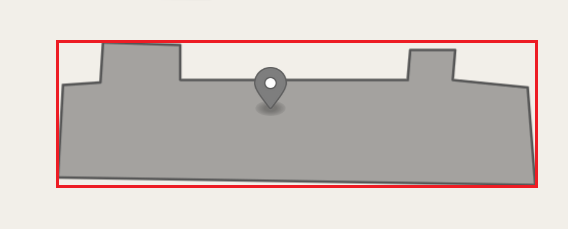
\includegraphics[width=0.9\textwidth]{./charpter1/my_home_bounds.png}
		      \end{figure}
	\end{itemize}
\end{note}



\section{投影变换}
投影变换是将真实的三维的椭球的地球显示投影成平面的二维地图上。
以国内常用的的二中投影来进行介绍:
\begin{enumerate}
	\item 等分弧秒投影
	\item 墨卡托投影(Mercator Projection)
	\item 高斯-克吕格投影(Transverse Mercator Projection)
\end{enumerate}
投影变换的本质是将\textbf{真实三维的(x, y, z) 投放到平面二维的(x, y)上}。

\subsection{墨卡托投影}
墨卡托的投影原理是正轴等角圆柱投影\footnote{https://en.wikipedia.org/wiki/Mercator\_projection}。
\begin{figure}[!htb]
	\centering
	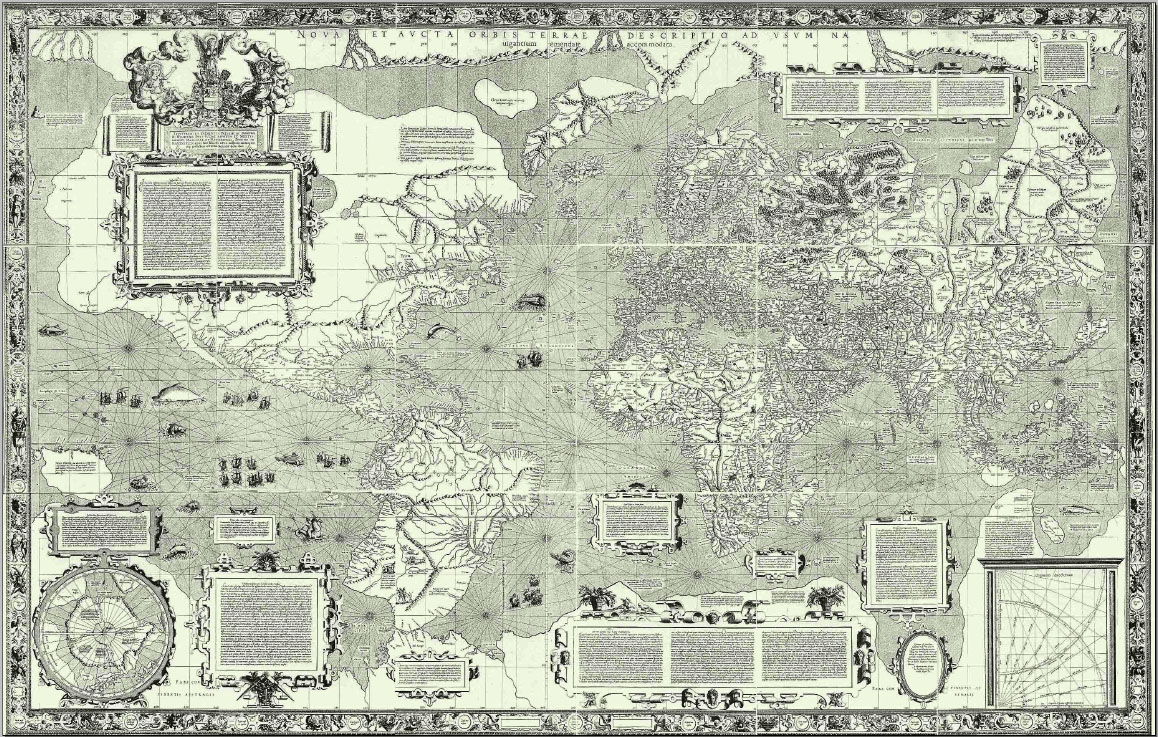
\includegraphics[width=0.9\textwidth]{./charpter1/Mercator_1569.png}
\end{figure}
1569年的墨卡托投影\footnote{https://en.wikipedia.org/wiki/Mercator\_1569\_world\_map}


\begin{figure}[!htb]
	\centering
	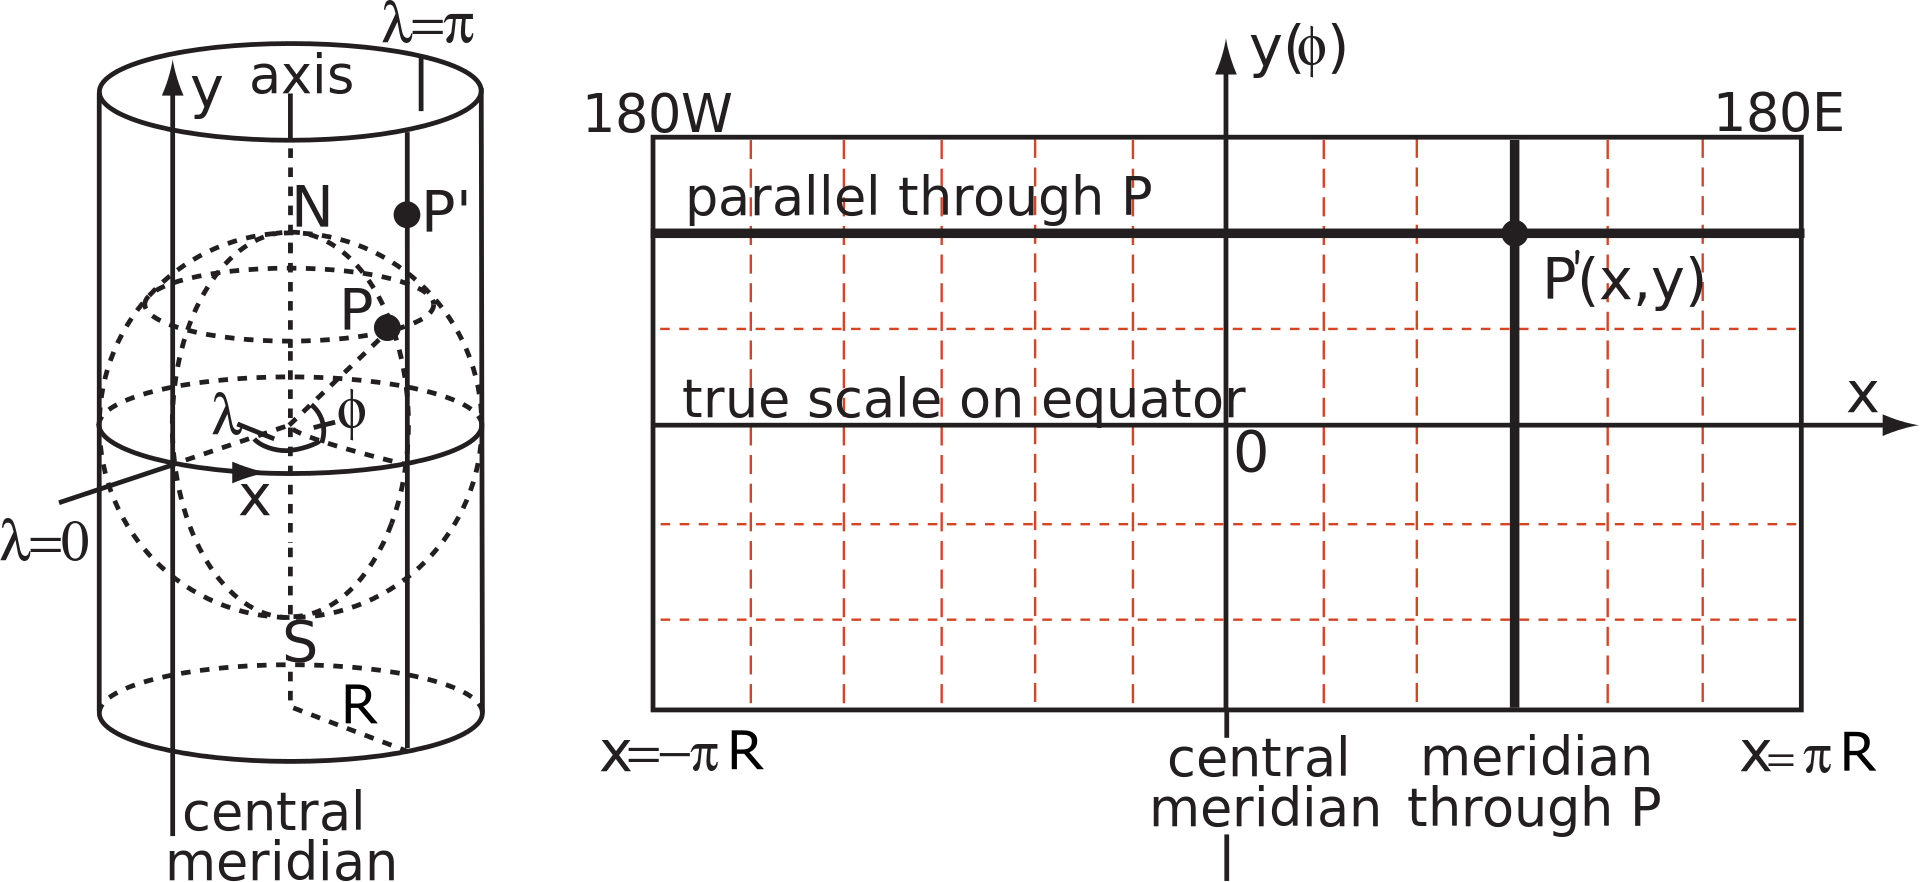
\includegraphics[width=0.9\textwidth]{./charpter1/Cylindrical_Projection_basics2.png}
\end{figure}
图中的一个实际地球表面上的点P经过投影变换后投射到圆柱平面上的点P'
\begin{enumerate}
	\item 经度λ:
	\item 纬度φ:
	\item x轴:经度经过投影函数x(λ)后计算得出对应的值
	\item y轴:纬度经过投影函数y(φ)后计算得出对应的值
\end{enumerate}

\begin{note}
	这里绝对不能把该场景想象从地心发射一条光线从P点穿透出来射到圆柱上形成点P',这个是错误的计算方式和思维模拟。
\end{note}

\subsection{高斯-克吕格投影}
高斯-克吕格投影的投影原理是等角横切椭圆柱投影。
TM\footnote{https://en.wikipedia.org/wiki/Transverse\_Mercator\_projection}
UTM\footnote{https://en.wikipedia.org/wiki/Universal\_Transverse\_Mercator\_coordinate\_system}
记得我在学习的时候,课本上讲解的都是类似西瓜皮的投影方式,当时只是从大概上了解了其原理。我相信和我一样有着疑问的人不在少数。本章节将从工程角度上详细剖解其数学原理。
\begin{figure}[!htb]
	\centering
	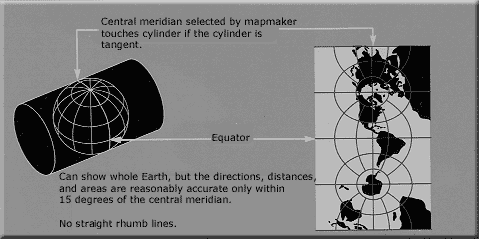
\includegraphics[width=0.9\textwidth]{./charpter1/Usgs_map_traverse_mercator.png}
\end{figure}



\section{切分模型}
由于一次性传输大量的矢量数据会导致性能瓶颈,因此需要针对海量数据进行LOD\footnote{多层次细节,Level Of Detail}处理.

\subsection{切分原理}
切分的基本原理是将整个世界
\begin{figure}[!htb]
	\centering
	% https://www.latexstudio.net/archives/51453.html
	% https://en.wikibooks.org/wiki/LaTeX/PGF/TikZ
	% https://graphviz.org/doc/info/shapes.html
	\begin{tikzpicture} [scale=2]
		\draw[step=1,color=gray!40] (-2,-1) grid (2,1);
		\draw[->] (-3,0) -- (3,0) node[right] {$x$};
		\draw[->] (0,-2) -- (0,2) node[right] {$y$};
		\draw[red] (10:1cm) (-2, 0) -- (2, 0) node[right] {赤道};
		\draw[blue] (10:1cm) (0,-1) -- (0,1) node[align=center] {本初子午线};
		\draw[dotted] (-2,1) node {西北 -180,90 };
		\draw[dotted] (2,1) node {东北 180, 90};
		\draw[dotted] (-2,-1) node {西南 -180 -90};
		\draw[dotted] (2,-1) node {东南 180 -90};
		\draw[dotted] (2,1) node {东北 180, 90};
		\draw[dashed, red, ->] (1,0.5) -- (1,0);
		\draw[dashed, blue, ->] (1,0.5) -- (0,0.5);
		\draw[dotted, red] (1,0.5) node {(90, 45)};
	\end{tikzpicture}
	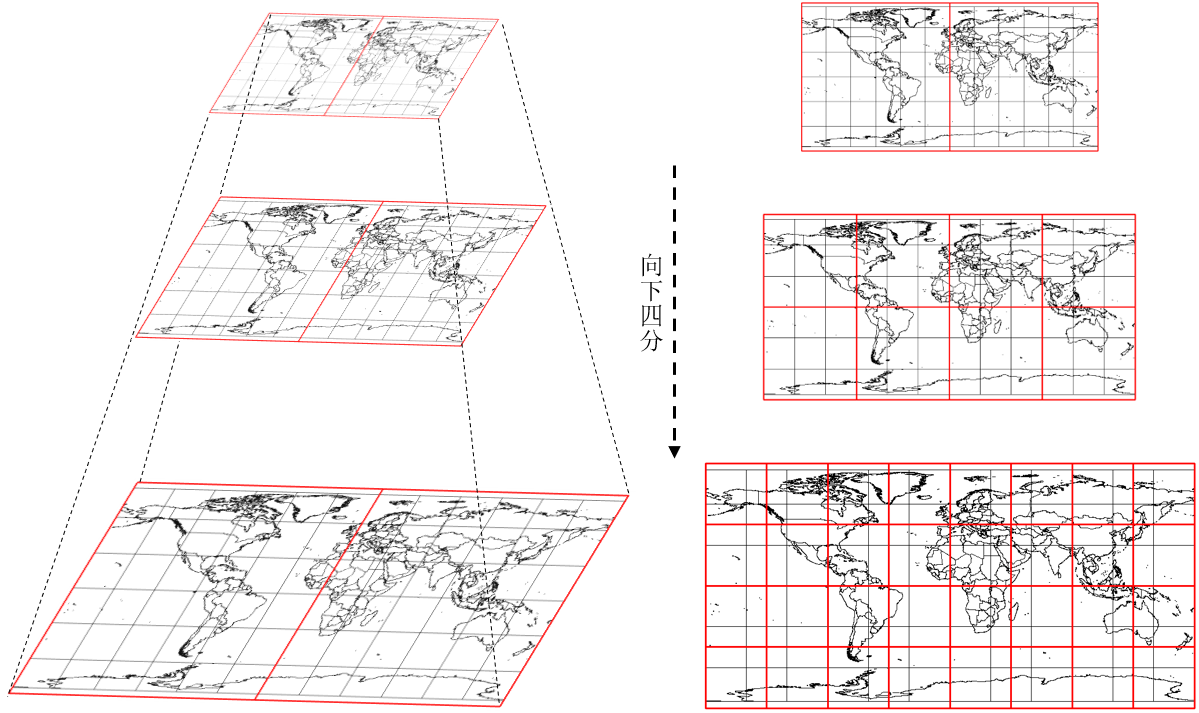
\includegraphics[width=0.9\textwidth]{./charpter1/lonlat_tilegrid.png}
\end{figure}

\subsection{切分规则}

瓦片矩阵集由多个瓦片矩阵集合组成,每个瓦片矩阵都有一个分辨率针对特定比例进行优化,并由\textbf{TileMatrix}标识符标识。
% 每个贴图矩阵集都有一个可选的近似边界框,但每个贴图矩阵都有间接从其他参数推导出的精确边界框。
瓷砖矩阵由于像素对齐,每个比例的包围框通常会略有不同对于客户机和服务器来说,考虑这种变化是很重要的。
在左上角瓷砖矩阵在CRS坐标中的点(tileMatrixMinX, tileMatrixMaxY),
宽度和瓦片矩阵的高度,以瓦片单位(matrixWidth, matrixHeight),
宽度和贴图的高度,以像素为单位(tileWidth, tileHeight),
转换坐标的系数参考系统(CRS)的单位分为米(metersPerUnit)
和比例尺(1: scalednominator),
贴图矩阵的边界框的右下角(tileMatrixMaxX, tileMatrixMinY)可计算如下:

OGC WMTS标准中DPI是90.71,即采用0.028mm作为一个像素的物理宽度,与天地图规范不一致(规范中DPI为96)。
前端程序调用WMTS接口获取元信息后,需要根据元信息中的比例尺和DPI参数重新计算瓦片分辨率。
理论上,天地图或支持天地图的相关产品DPI值都应该为96。
ArcGIS等商业软件的DPI值默认采用OGC标准中的90.71。


DPI(每英寸多少像素点) = dots / inch  = 90.71 dpi; \\
1 英寸 = 25.4 毫米 \\
DPMM(每毫米多少像素点) = dots / millimeter =  DPI * (millimeter / inch) = 25.4 / 90.71 = 0.28;

\begin{align}
	scale = 1 inch                                                    \\
	pixelSpan = scaleDenominator \times 0.28 \div metersPerUnit(crs); \\
	tileSpanX = tileWidth \times pixelSpan;                           \\
	tileSpanY = tileHeight \times pixelSpan;                          \\
	tileMatrixMaxX = tileMatrixMinX + tileSpanX \times matrixWidth;   \\
	tileMatrixMinY = tileMatrixMaxY - tileSpanY \times matrixHeight;
\end{align}

\begin{figure}[!htb]
	\centering
	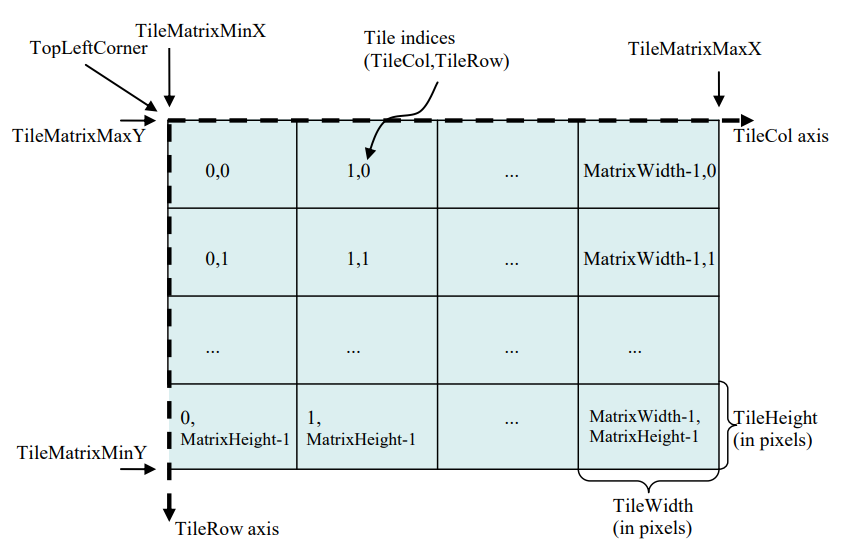
\includegraphics[width=0.55\textwidth]{./charpter1/ogc_tilegrid.png}
	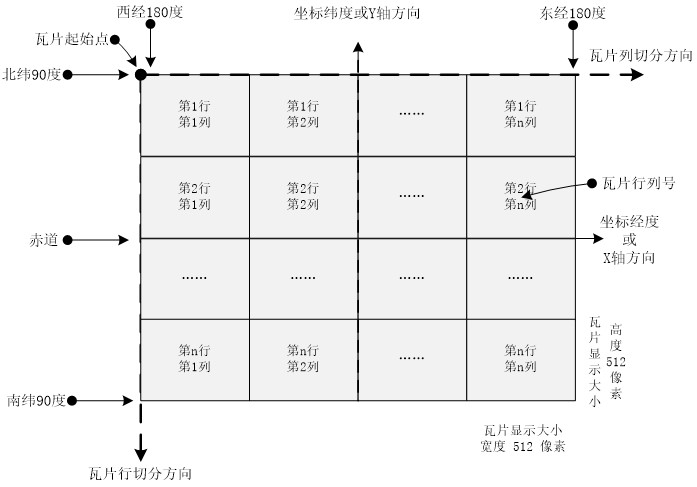
\includegraphics[width=0.55\textwidth]{./charpter1/math_tilegrid.jpg}
\end{figure}

\subsection{常见切分规范}
\begin{itemize}
	\item EPSG:4326 等分弧秒投影 \footnote{地理坐标系统(Geographical Coordinate System), 经纬度直投, 近似是说的同一个东西,这里该投影属于一种任意投影,不太严谨,不做学术上争论 , http://epsg.io/4326}
	\item EPSG:3857 Web墨卡托投影 \footnote{投影坐标系统 (Projection Coordinate System) http://epsg.io/3857}
\end{itemize}

\subsubsection{等分弧秒投影}
\label{sec:lonlat-project}
经纬度等分弧秒投影后的世界地图为南北短,东西宽的矩形。选择在经度0方向进行切割,使得全球地图是两张在经纬度方向长宽相等的正方形矩形区域。全球制图范围为纬度 [-90, 90],经度[-180, 180]。
\begin{itemize}
	\item Cesium地形\footnote{\hyperref[sec:cesium-terrain]{跳转至Cesium地形章节}}默认采取该投影
	\item Cesium栅格\footnote{\hyperref[sec:cesium-raster]{跳转至Cesium栅格章节}}可以通过\textbf{GeographicTilingScheme}加载经纬度坐标系瓦片
\end{itemize}

\begin{figure}[!htb]
	\centering
	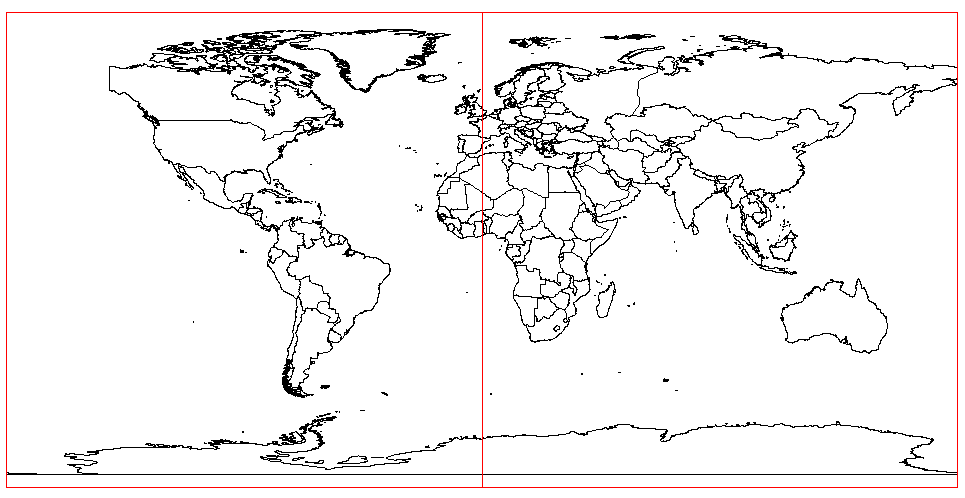
\includegraphics[width=0.8\textwidth]{./charpter1/tile/lonlat-level-1.png}
\end{figure}
\subsubsection{Web墨卡托投影}
Web墨卡托投影后的世界地图为南北略长,东西略窄的矩形,选择在纬度+-85.051128度进行切割,使得全球地图是一张在经纬度方向长宽相等的正方形区域。此时全球制图范围为纬度[-85.051128, 85.051128], 经度[-180, 180],投影后平面坐标范围为:X[-20037508.34米, 20037508.34米], Y[-20037508.34米, 20037508.34米]。
\hyperref[sec:cesium-terrain]{Cesium栅格默认采取该投影}
\begin{itemize}
	\item Cesium栅格\footnote{\hyperref[sec:cesium-raster]{跳转至Cesium栅格章节}}默认采取该投影
	\item MapboxGL栅格默认采取该投影
\end{itemize}
\begin{figure}[!htb]
	\centering
	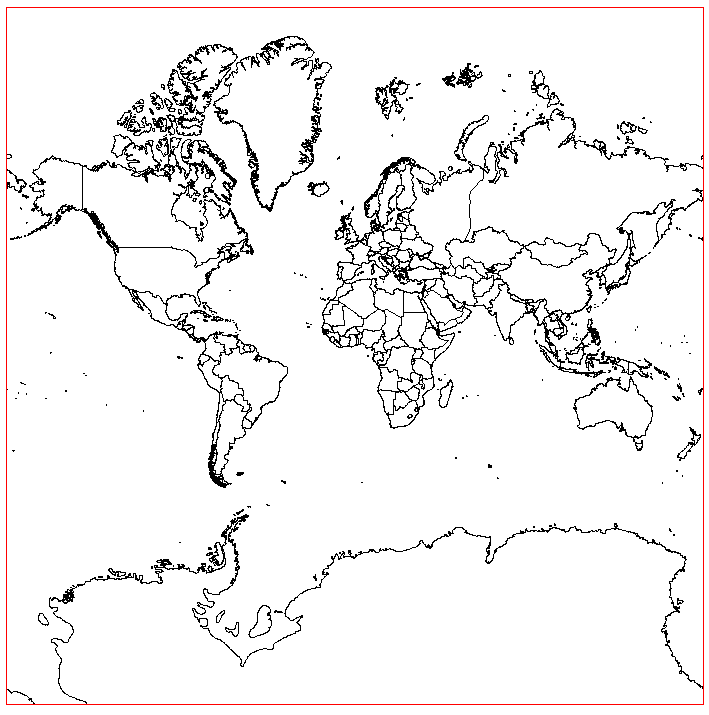
\includegraphics[width=0.5\textwidth]{./charpter1/tile/mkt-level-1.png}
\end{figure}
\subsubsection{投影组合}
\textbf{Cesium投影组合}

\begin{introduction}
	\item Cesium地形\textbf{默认采取等分弧秒投影}
	\item Cesium栅格\textbf{默认采取Web墨卡托投影}
	\item 投影坐标直接叠加显示 ? 否
	\item 矩阵变换叠加显示 ? 是
\end{introduction}
不知道细心的读者有没有上2章的细节中发现一个现象。那如果都走默认的前提下,岂不是2种投影叠加到一起的显示方式吗?
\begin{figure}[!htb]
	\centering
	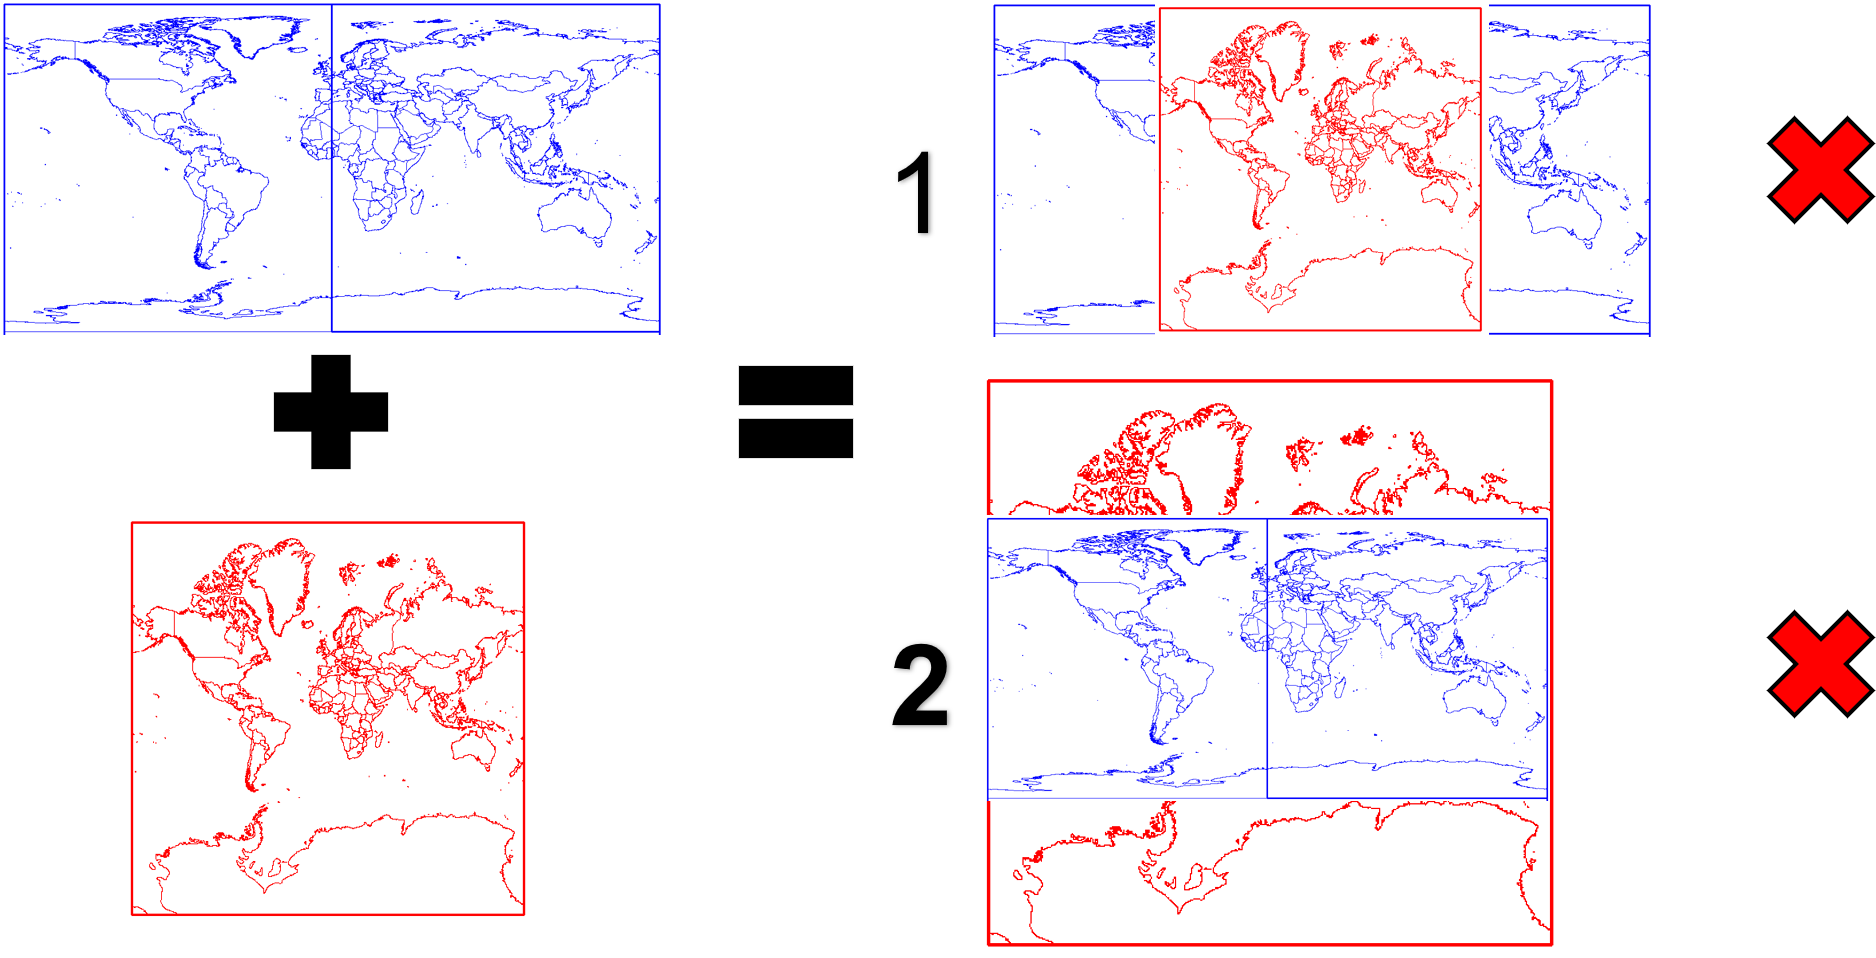
\includegraphics[width=1.0\textwidth]{./charpter1/project/error_combine.png}
\end{figure}
\begin{note}
	如上图所示,两种方式都无法通过简单的平移或者拉伸的方式来套合在一起。
\end{note}

\textbf{MapboxGL投影组合}

\section{变换}
上一节的投影讲解了如何把一个三维球形的投影到二维的平面上。但是实际场景中,可能需要进行一些放大,平移,旋转操作。
\begin{note}
	这一系列类操作在WebGL中通常称作模型变换。
\end{note}

\begin{enumerate}
	\item 放大操作,以某点为中心,按照比例进行缩放。
	\item 平移操作,以某点为中心,按照距离进行平移。
	\item 旋转操作,以某点为中心,按照角度进行旋转。
	\item 组合以上3中操作。
\end{enumerate}

\subsection{旋转操作}

\begin{SCfigure}
	\centering
	\caption{原始图像.左图如果是呈现在屏幕上,由于绝大部分的屏幕是宽大于高,因此该图形的左右侧会出现很多的空隙,
		因此在观感上表现会很稀疏。因此如果能够把该图形旋转90度后横着放,就可以省下很多的空间了。
		那如何旋转呢,是以左上角还是右上角还是左下角还是右上角呢,这里我们先选择最容易理解的中心点来演示。
		图中的绿色点表示中心点。}
	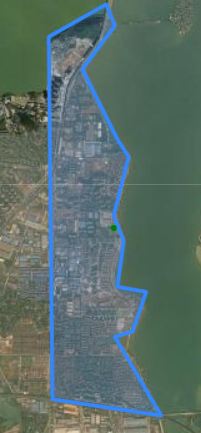
\includegraphics[width=0.3\textwidth]{./charpter1/transform/before_rotate.png}
\end{SCfigure}

\begin{figure}[!htb]
	\centering
	\caption{旋转后的位置如图所示}
	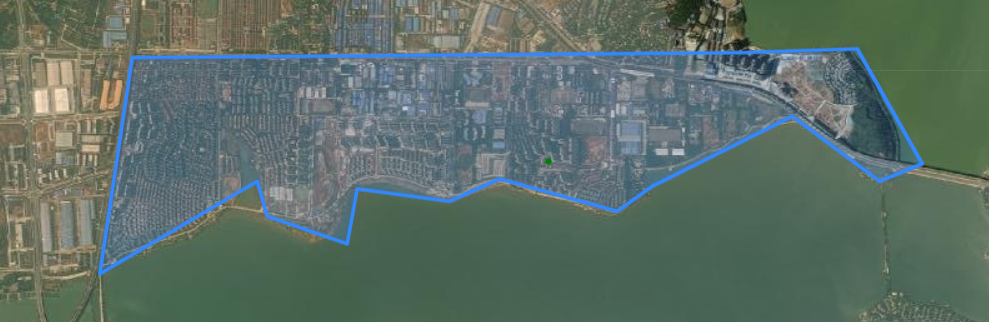
\includegraphics[width=0.8\textwidth]{./charpter1/transform/after_rotate.png}
\end{figure}

\subsection{数学原理}
\begin{figure}[!htb]
	\centering
	\caption{图形原理}
	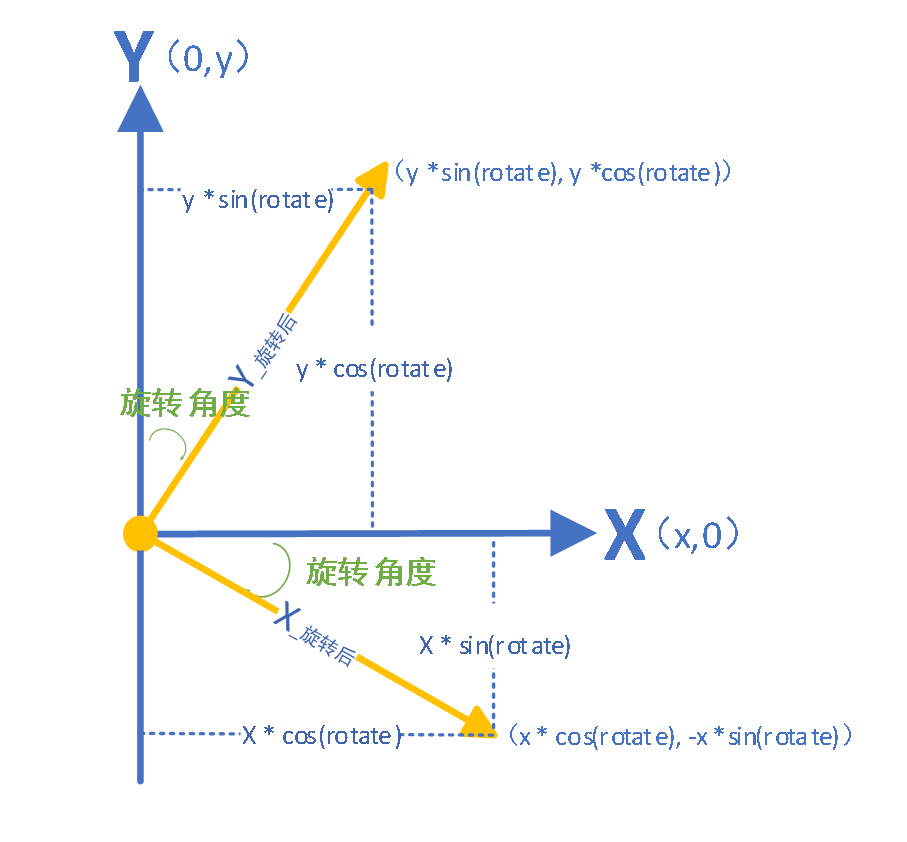
\includegraphics[width=0.8\textwidth]{./charpter1/transform/rotate.png}
\end{figure}

上图可以知道得到的原来的正常的的X,Y通过旋转角度 $\alpha$ 后得到的新的$X'$, $Y'$如下所示:

\begin{subequations}
	\begin{align}
		X & =(x, 0) \\
		Y & =(0, y)
	\end{align}
\end{subequations}

\begin{subequations}
	\begin{align}
		X' & =(x \times \cos \alpha, -x \times \sin \alpha) \\
		Y' & =(y \times \sin \alpha, y \times \cos \alpha)
	\end{align}
\end{subequations}

上面的公式知道了原始的X,Y的基向量,也求出了旋转后的X',Y'的基向量。
因此原始X,Y中的向量$\overrightarrow{A}$,在新坐标系X',Y'后得到的$\overrightarrow{A'}$值为
	\begin{subequations}
		\begin{align}
			\overrightarrow{A} & = (a, b) \\
			X' & =(x \times \cos \alpha, -x \times \sin \alpha) \\
			Y' & =(y \times \sin \alpha, y \times \cos \alpha)
		\end{align}
	\end{subequations}

	\begin{subequations}
		\begin{align}
		\overrightarrow{A'} = \begin{bmatrix}X' \\ Y'\end{bmatrix} \times \overrightarrow{A}
		 = \begin{bmatrix} 
			\cos \alpha & \sin \alpha \\
			- \sin \alpha & \cos \alpha
		 \end{bmatrix} \times \begin{bmatrix} a \\ b \end{bmatrix}   
		 = a \times \begin{bmatrix}  \cos \\ - \sin \end{bmatrix} + b \times \begin{bmatrix}  \sin \\ \cos \end{bmatrix} 
		 = \begin{bmatrix}
			\frac{5}{6} & \frac{1}{6} & 0
			\\[0.3em]
			\frac{5}{6} & 0
			& \frac{1}{6} \\[0.3em]
			0
						& \frac{5}{6} & \frac{1}{6}
	\end{bmatrix}
	\end{align}
  \end{subequations}
\chapter{Cesium代码解析}

\section{基本原理}
\begin{enumerate}
	\item 初始状态:从太空中远眺地球,将看到的地球三维场景绘制在平面画布上。每秒保持60帧的频率不断渲染画布。
	      \begin{figure}[!htb]
		      \centering
		      
\includegraphics[width=0.6\textwidth]{./charpter2/base/global.png}
	      \end{figure}
	\item 交互状态:当用户人机交互(放大/缩小)改变了视角后,由于每一帧都会重绘画布,让用户感觉是自己主动更新了画布一般,实际上是通过高频率的被动渲染来实现的。
\end{enumerate}

\subsection{核心代码}

\begin{enumerate}
	\item 轮询主入口 Source/Core/\textbf{requestAnimationFrame.js}。这个是封装js自身的requestAnimationFrame.js的requestAnimationFrame的缺陷在于只能通过window上下文来invoke回调,需要实现一种脱离window上下文的封装。
	\item 场景组件 Source/Widgets/CesiumWidget/\textbf{CesiumWidget.js} 用来呈现三维球场景的DOM场景组件。
	      \begin{figure}[!htb]
		      \centering
		      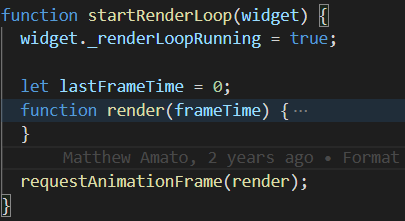
\includegraphics[width=0.5\textwidth]{./charpter2/base/loop.png}
	      \end{figure}
	      \begin{enumerate}
		      \item 构造函数内部逻辑
		            \begin{enumerate}
			            \item 初始化规定的椭球Ellipsoid,默认是WGS84
			            \item 初始化天空盒、月亮、太阳、大气环境
			            \item 初始化基本的栅格底图
			            \item 初始化基本的地形
			            \item 执行核心渲染进程,启动每秒60帧的轮询进程
		            \end{enumerate}

	      \end{enumerate}
	\item 核心渲染进程 Source/Scene/\textbf{Scene.js}
	      \begin{enumerate}
		      \item 先进入Scene的initializeFrame以及render函数
		      \item 先进入Scene的render函数是整个场景的主入口,内部会进行对应的各种不同图层的任务分发与调度,代码如下所示
		            \begin{lstlisting}
scene.globe.beginFrame(frameState); // 一帧的开始

scene.updateEnvironment();
// 只考虑球面模式实际是executeCommandsInViewport在工作
scene.updateAndExecuteCommands(passState, backgroundColor); 
scene.resolveFramebuffers(passState);

passState.framebuffer = undefined;
executeOverlayCommands(scene, passState);

scene.globe.endFrame(frameState); // 一帧的结束
\end{lstlisting}
	      \end{enumerate}
	\item 地形渲染 Source/Scene/\textbf{Globe.js}
	      \begin{enumerate}
		      \item 地形渲染的入口是Globe.js,其核心的工作类是surface,其构造函数如下:
		            \begin{lstlisting}
			// 默认采取四叉树构建表面	
			this._surface = new QuadtreePrimitive({ 
				tileProvider: new GlobeSurfaceTileProvider({
					terrainProvider: terrainProvider, // 一份地形
					imageryLayers: imageryLayerCollection, // 一组栅格瓦片底图
					surfaceShaderSet: this._surfaceShaderSet
				})
			});
		\end{lstlisting}
		      \item 地形的渲染是通过Globe.render beginFrame endFrame,三者共同组成其声明周期。
		            \begin{enumerate}
			            \item \textbf{beginFrame}函数原理
			                  \begin{lstlisting}
				QuadtreePrimitive.prototype.beginFrame = function (frameState) {
					var passes = frameState.passes;
					if (!passes.render) {
						return;
					}
				
					if (this._tilesInvalidated) {
						invalidateAllTiles(this);
						this._tilesInvalidated = false;
					}
				
					// Gets commands for any texture re-projections
					this._tileProvider.initialize(frameState);
				
					clearTileLoadQueue(this);
				
					if (this._debug.suspendLodUpdate) {
						return;
					}
				
					this._tileReplacementQueue.markStartOfRenderFrame();
				};
			\end{lstlisting}
			                  \begin{tikzpicture}
				                  \begin{umlseqdiag}
					                  \umlobject[class=Scene]{S}
					                  \umlobject[class=Globe]{G}
					                  \umlobject[class=QuadtreePrimitive]{surface}
					                  \umlobject[class=GlobeSurfaceTileProvider]{t}
					                  \begin{umlcall}{S}{G}
						                  \begin{umlcall}[op=beginFrame(),type=synchron,return=0]{G}{surface}
							                  \begin{umlcall}[type=synchron,fill=green]{surface}{t}
								                  \begin{umlcallself}[op=setTerrainProvidertype=synchron,fill=green]{t}
								                  \end{umlcallself}
							                  \end{umlcall}
							                  \begin{umlcallself}[op=start-beginFrame,type=synchron,fill=blue,return=end-beginFrame]{surface}
								                  \begin{umlcall}[op=initialize,type=synchron,fill=blue]{surface}{t}
								                  \end{umlcall}
								                  \begin{umlcallself}[op=clearTileLoadQueue,type=synchron,fill=blue]{surface}
								                  \end{umlcallself}
								                  \begin{umlcallself}[op=markStartOfRenderFrame,type=synchron,fill=blue]{surface}
								                  \end{umlcallself}
							                  \end{umlcallself}
						                  \end{umlcall}
					                  \end{umlcall}
				                  \end{umlseqdiag}
			                  \end{tikzpicture}
			            \item \textbf{render}函数原理
			                  \begin{lstlisting}
							QuadtreePrimitive.prototype.render = function (frameState) {
							var passes = frameState.passes;
							var tileProvider = this._tileProvider;

							if (passes.render) {
								tileProvider.beginUpdate(frameState);

								selectTilesForRendering(this, frameState);
								createRenderCommandsForSelectedTiles(this, frameState);

								tileProvider.endUpdate(frameState);
							}

							if (passes.pick && this._tilesToRender.length > 0) {
								tileProvider.updateForPick(frameState);
							}
						};
						\end{lstlisting}
			                  \begin{tikzpicture}
				                  \begin{umlseqdiag}
					                  \umlobject[class=Scene]{S}
					                  \umlobject[class=Globe]{G}
					                  \umlobject[class=QuadtreePrimitive]{surface}
					                  \umlobject[class=GlobeSurfaceTileProvider]{t}
					                  \begin{umlcall}{S}{G}
						                  \begin{umlcall}[op=render(),type=synchron,return=0]{G}{surface}
							                  % \begin{umlcall}[type=synchron,fill=green]{surface}{t}
							                  % 	\begin{umlcallself}[op=setTerrainProvidertype=synchron,fill=green]{t}
							                  % 	\end{umlcallself}
							                  % \end{umlcall}
							                  \begin{umlcallself}[op=start-render,type=synchron,fill=blue,return=end-render]{surface}
								                  \begin{umlcall}[type=synchron,fill=yellow]{surface}{t}
									                  \begin{umlcallself}[op=beginUpdate,type=synchron,fill=green]{t}
									                  \end{umlcallself}
								                  \end{umlcall}
								                  \begin{umlcallself}[op=selectTilesForRendering,type=synchron,fill=blue]{surface}
								                  \end{umlcallself}
								                  \begin{umlcallself}[op=createRenderCommandsForSelectedTiles,type=synchron,fill=blue]{surface}
								                  \end{umlcallself}
								                  \begin{umlcall}[type=synchron,fill=yellow]{surface}{t}
									                  \begin{umlcallself}[op=endUpdate,type=synchron,fill=green]{t}
									                  \end{umlcallself}
								                  \end{umlcall}
							                  \end{umlcallself}
						                  \end{umlcall}
					                  \end{umlcall}
				                  \end{umlseqdiag}
			                  \end{tikzpicture}
			            \item \textbf{endFrame}函数原理
		            \end{enumerate}
	      \end{enumerate}
\end{enumerate}

\section{地形}
\label{sec:cesium-terrain}
地形在采集的时候,大部分都是通过经纬度+高度灰度值的方式采集的。Cesium默认的地形的加载策略也是经纬度。在实际显示的时候是将地形作为基础结构显示在三维场景中。
\begin{figure}[!htb]
	\centering
	\begin{subfigure}[b]{0.58\textwidth}
        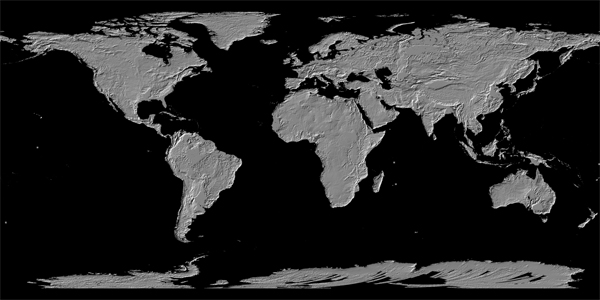
\includegraphics[width=\textwidth]{./charpter2/terrian/world_dem_2d.jpg}
        \caption{平面经纬度地形}
        \label{fig:world_dem_2d}
    \end{subfigure}
    \begin{subfigure}[b]{0.3\textwidth}
		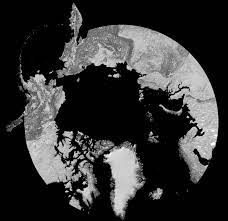
\includegraphics[width=\textwidth]{./charpter2/terrian/world_dem_3d.jpg}	
        \caption{球面经纬度地形}
        \label{fig:world_dem_3d}
    \end{subfigure}
\end{figure}

\begin{introduction}
	\item 那如何将平面的地形贴合到球面呢?
	\item 直接使用极坐标?
	\item 间接使用笛卡尔积坐标?
\end{introduction}

\subsection{椭球基本知识}
\begin{enumerate}
	\item 基本方程 
	\begin{equation}
		\frac{x^2}{a^2} + \frac{y^2}{b^2} + \frac{z^2}{c^2} = 1
	\end{equation}
	\item 扁率\footnote{扁率e = (a – c) / a = 1 / 298.257223563, 很多时候喜欢使用分母298来表示扁率}
	\begin{equation}
		e = \frac{a - c}{a} 
	\end{equation}
	\item 扁率以及长短轴的互相计算
	\begin{equation}
		c = a * (1 - e)
	\end{equation}
\end{enumerate}	


\begin{figure}[!htb]
	\centering
	\begin{subfigure}[b]{0.4\textwidth}
        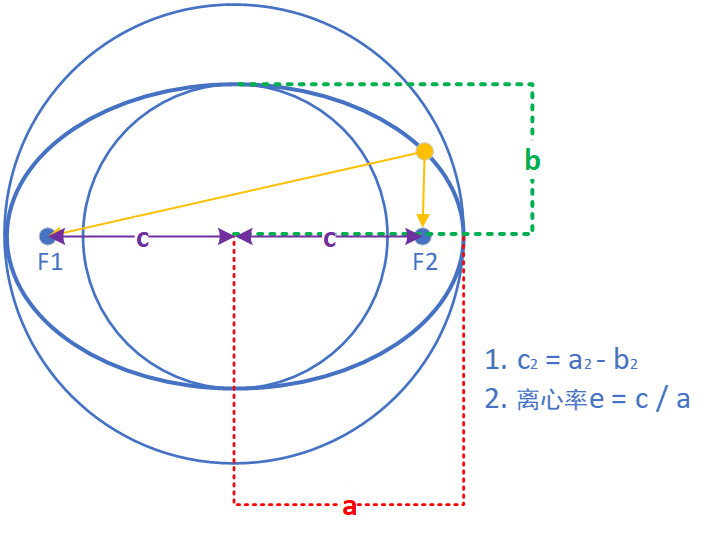
\includegraphics[width=\textwidth]{./charpter2/terrian/ellipsoid.png}
        \caption{椭圆基本理论知识}
    \end{subfigure}
    \begin{subfigure}[b]{0.5\textwidth}
		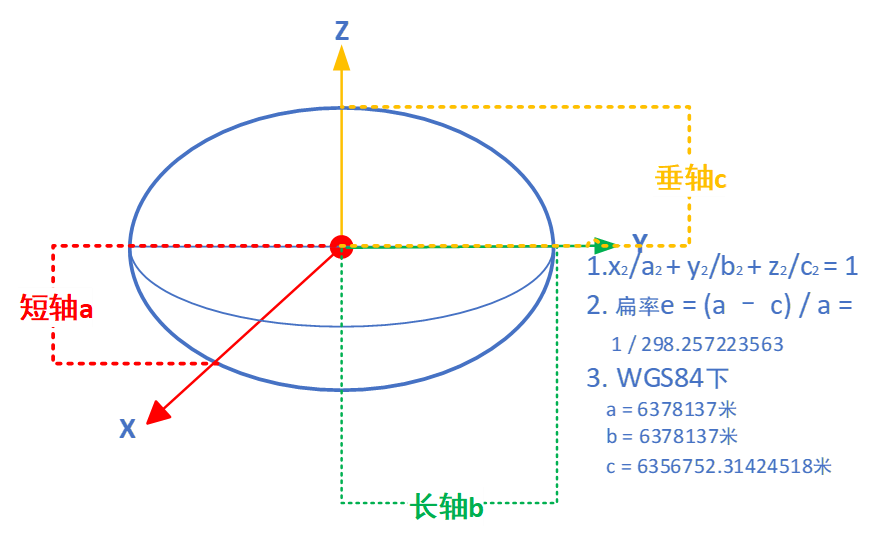
\includegraphics[width=\textwidth]{./charpter2/terrian/ellipsoid_wgs84.png}	
        \caption{椭球基本理论知识}
    \end{subfigure}
\end{figure}

\subsection{地形核心原理}
核心原理是先根据经纬度计算出\hyperref[sec:ellipsoid-surface]{\textbf{椭球表面}}上一个点对应的笛卡尔积,然后再追加加该点对应的高度h的向量,就可以得到椭球坐标系下\hyperref[sec:ellipsoid-dem-height]{\textbf{地形高程}}的真实迪卡坐标值。
\begin{note}
	这段话开始不理解没关系,后面会极为详细的解析对应的空间原理
\end{note}
\begin{figure}[!htb]
	\centering
	\begin{subfigure}[b]{0.4\textwidth}
        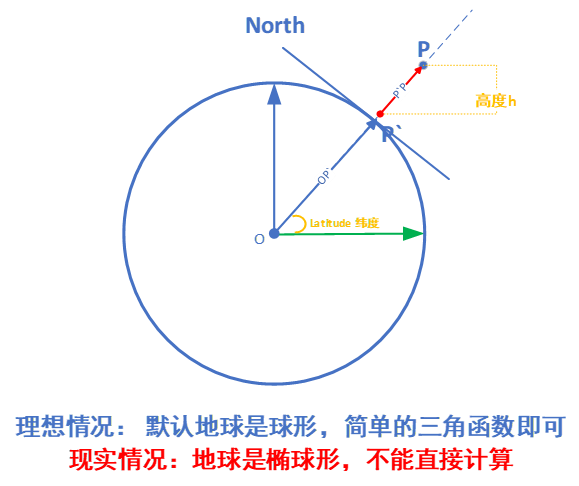
\includegraphics[width=\textwidth]{./charpter2/terrian/idea_state.png}
        \caption{理想情况}
        \label{fig:idea_state}
    \end{subfigure}
    \begin{subfigure}[b]{0.5\textwidth}
		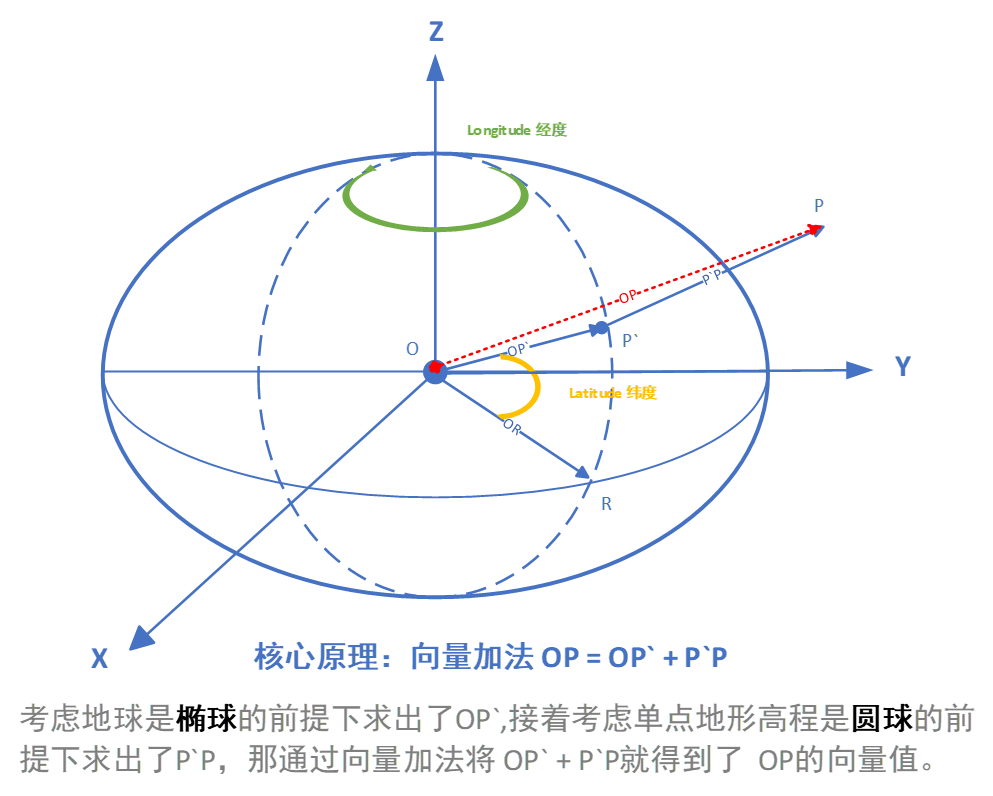
\includegraphics[width=\textwidth]{./charpter2/terrian/actual_state.png}	
        \caption{现实情况}
        \label{fig:actual_state}
    \end{subfigure}
\end{figure}

\subsection{椭球表面原理}
\label{sec:ellipsoid-surface}

\begin{figure}[!htb]
	\centering
	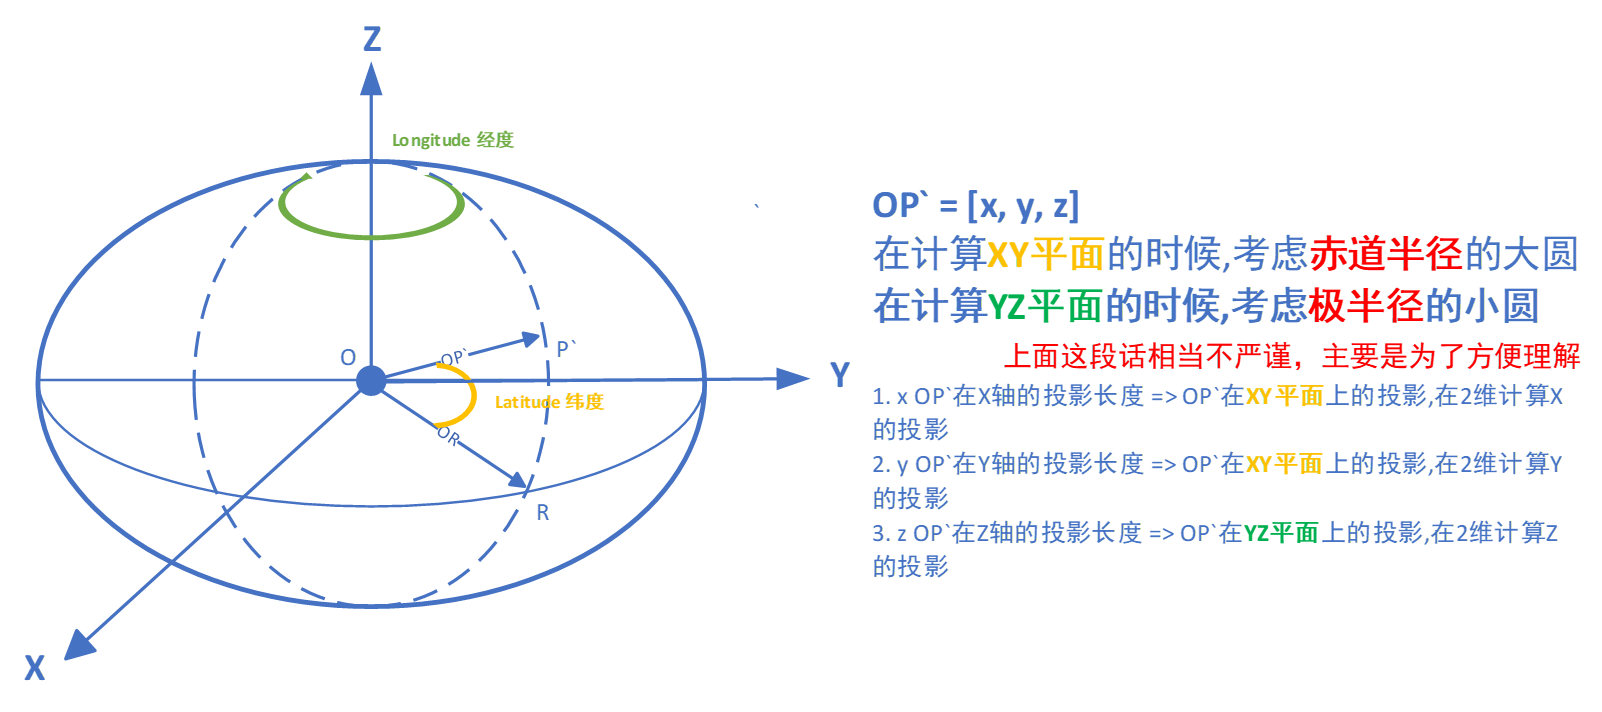
\includegraphics[width=1.0\textwidth]{./charpter2/terrian/ellipsoid_surface_xyz.png}
\end{figure}

\subsubsection{赤道半径平面计算}
\begin{figure}[!htb]
	\centering
	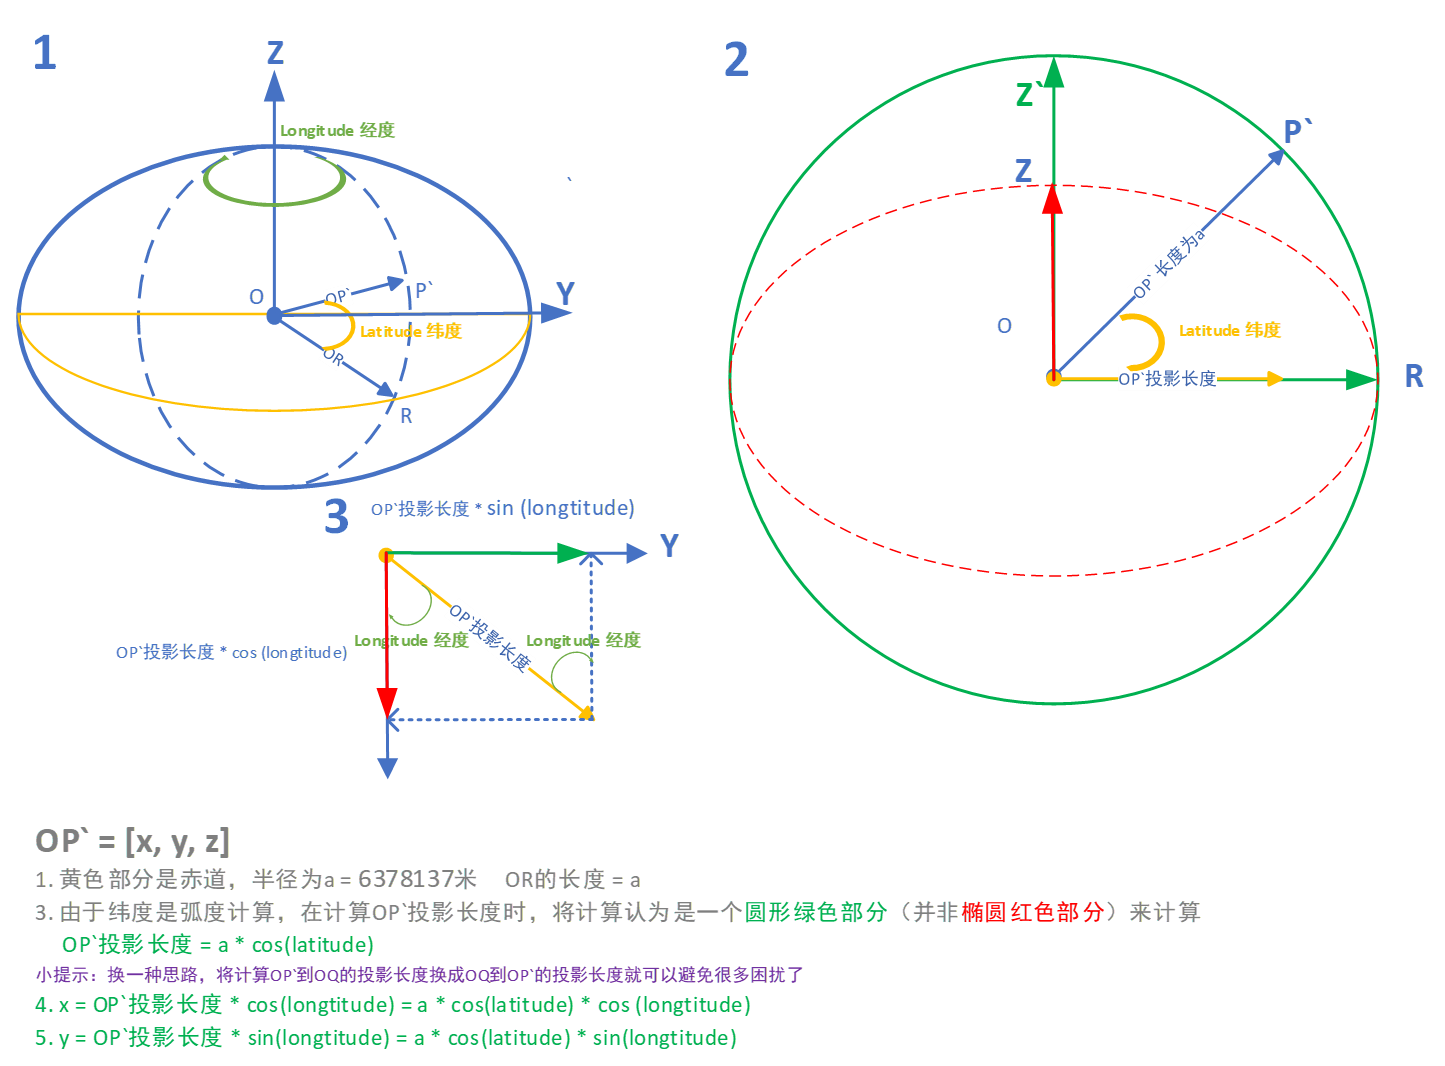
\includegraphics[width=1.0\textwidth]{./charpter2/terrian/ellipsoid_surface_equator.png}
\end{figure}
\subsubsection{极半径平面计算}
\begin{figure}[!htb]
	\centering
	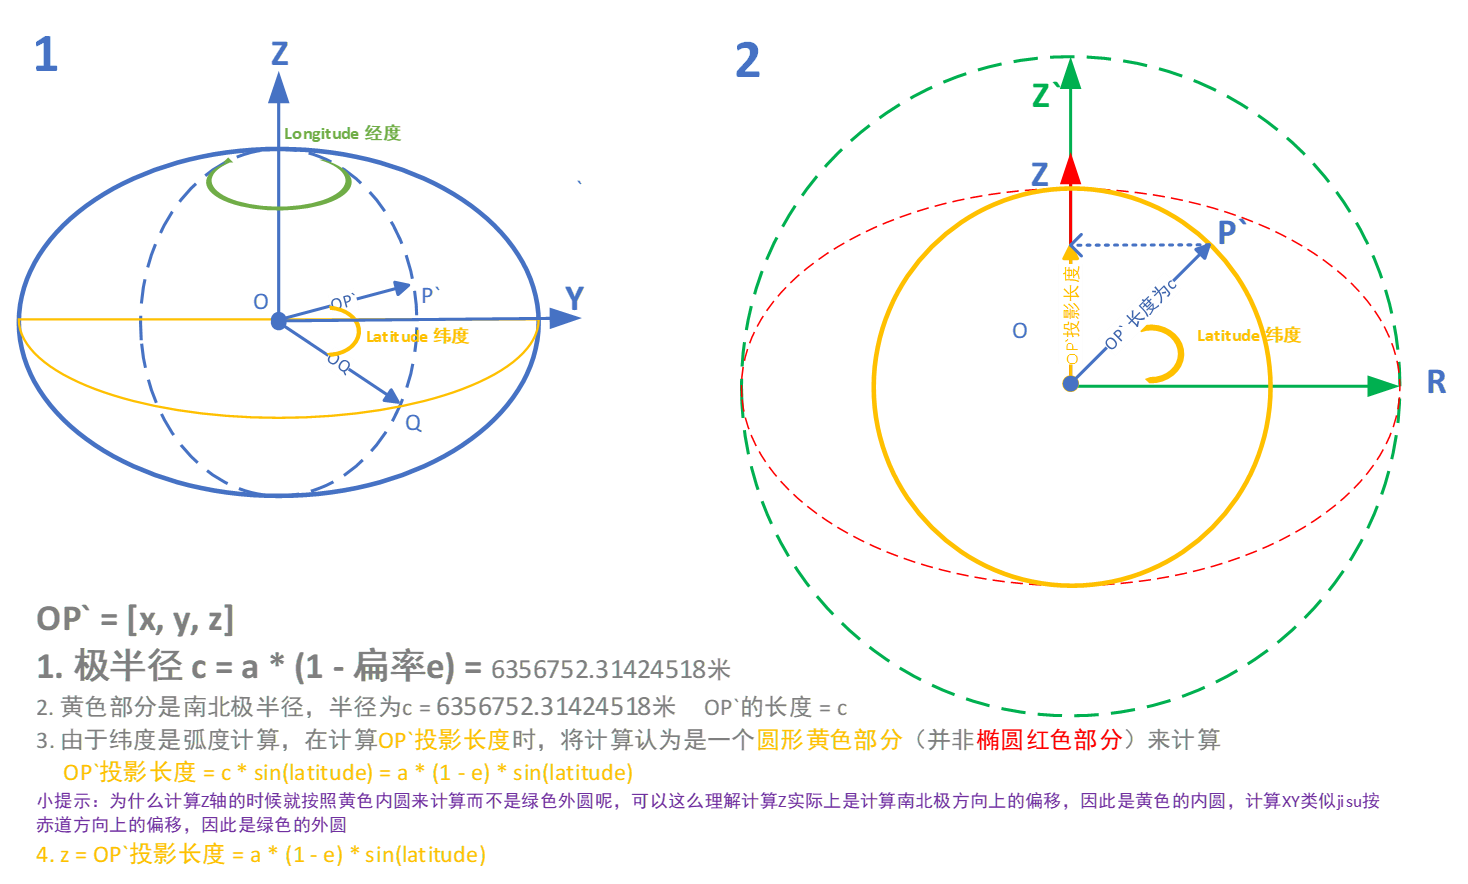
\includegraphics[width=1.0\textwidth]{./charpter2/terrian/ellipsoid_surface_pole.png}
\end{figure}

\subsection{地形高程原理}
\label{sec:ellipsoid-dem-height}
\begin{figure}[!htb]
	\centering
	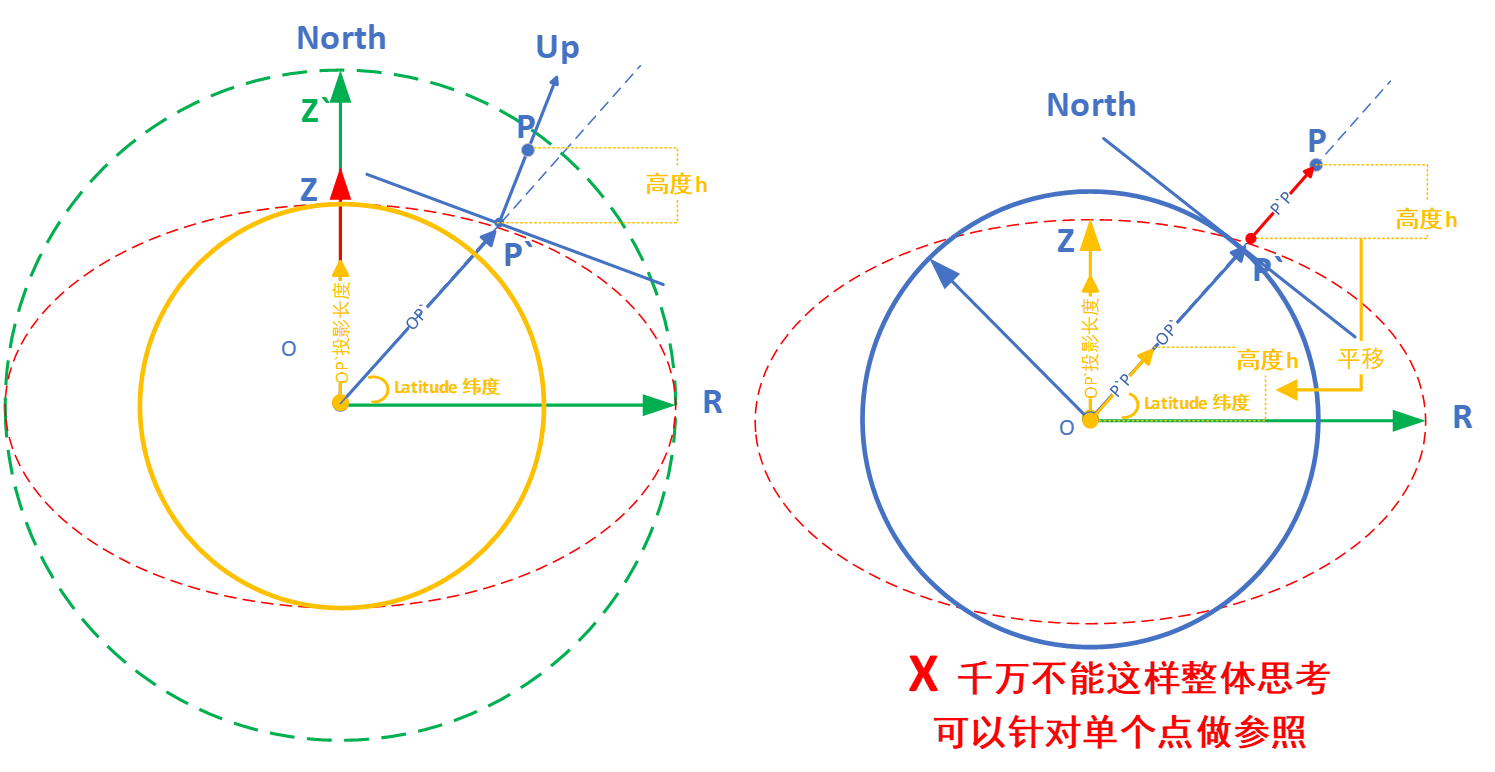
\includegraphics[width=1.0\textwidth]{./charpter2/terrian/ellipsoid_dem_height_1.png}
\end{figure}

\begin{equation}
	\overrightarrow{P'P} = \begin{bmatrix} x \\[0.3em] y \\[0.3em] z  \end{bmatrix} 
\end{equation}
\begin{enumerate}
	\item 之前计算OP'是把地球当作一个椭球来计算的得到的公式如下:
	\begin{enumerate}
		\item x = 赤道半径 * cos(longtitude) = a * cos(latitude) * cos (longtitude)
		\item y = 赤道半径 * sin(longtitude) = a * cos(latitude) * sin(longtitude)
		\item z = 极半径 * sin(latitude) = a * (1 - e) * sin(latitude)
	\end{enumerate}
	\item 现在我们思考一下,地球是一个椭球,某个点对应地形的高度在采集时候实际上是认为该点对应地表向下延申直至地心,其经纬度都和改地表点保持一致。在只考虑单点以及对应的参心圆球前提下,将红色P'P平移到黄色P'P上,就可以直接套用上面的公式
	\begin{enumerate}
		\item x = 地形高度 * cos(longtitude)  = h * cos(latitude) * cos (longtitude)
		\item y = 地形高度 * sin (longtitude)  = h * cos(latitude) * sin (longtitude)
		\item z = 地形高度 * sin (latitude)       = h * sin(latitude)
	\end{enumerate}
	\item 之前通过考虑地球是椭球的前提下求出了OP',接着考虑单点地形高程是圆球的前提下求出了P'P,那通过向量加法将 OP' + P'P就得到了  OP的向量值。
	\item 此时OP的物理意义是考虑地球是椭球的客观前提下,计算出来的地形对应的其在椭球坐标系下的笛卡尔坐标值。
\end{enumerate}

\subsection{公式汇总}
\begin{enumerate}
	\item lat = latitude = 纬度
	\item lng = longtiude = 经度
	\item e = 扁率
	\item a = 长轴(赤道半径) = 6378137米
	\item c = 短轴(极半径) = 6356752.31424518米
	\item h = height = 地形高度(每个点对应的地形灰度值都各不相同)
\end{enumerate}

\begin{equation}
	\overrightarrow{OP'} = \begin{bmatrix} x \\[0.3em] y \\[0.3em] z  \end{bmatrix} = 
	\begin{bmatrix} a \times{} \cos{lat} \times{} \cos{lng}  \\[0.3em]
	a \times{} \cos{lat} \times{} \sin{lng} \\[0.3em]
	a \times{} ( 1 - e) \times{} \sin{lat} \end{bmatrix}	
\end{equation}
\begin{equation}
	\overrightarrow{P'P} = \begin{bmatrix} x \\[0.3em] y \\[0.3em] z  \end{bmatrix} = 
	\begin{bmatrix} h \times{} \cos{lat} \times{} \cos{lng}  \\[0.3em]
	h \times{} \cos{lat} \times{} \sin{lng} \\[0.3em]
	h \times{} \sin{lat} \end{bmatrix}	
\end{equation}	
\begin{equation}
	\overrightarrow{OP} = \overrightarrow{OP'} + \overrightarrow{P'P} = 
	\begin{bmatrix} (a + h) \times{} \cos{lat} \times{} \cos{lng}  \\[0.3em]
		(a + h) \times{} \cos{lat} \times{} \sin{lng} \\[0.3em]
		(a \times{} ( 1 - e) + h) \times{} \sin{lat} \end{bmatrix}	
\end{equation}	

\subsection{生命周期}
\begin{introduction}
	\item 基础框架生命周期
	\item MapGIS地形如何在基础生命周期中工作?
	\item STK地形如何在基础生命周期中工作?
\end{introduction}

\textbf{基础框架生命周期}

\begin{enumerate}
	\item QuadtreePrimitive.processSinglePriorityLoadQueue();
	\item GlobeSurfaceTileProvider.loadTile();
	\item GlobeSurfaceTile.processStateMachine()->requestTileGeometry()->doRequest()
	\item requestPromise = terrainProvider.requestTileGeometry(x, y, level, request); 这一步的terrainProvider使用初始化的地形,如果是IGS就是MapGISTerrainProvider。
\end{enumerate}

\begin{tikzpicture}
	\begin{umlseqdiag}
		\umlobject[class=QuadtreePrimitive]{QT}
		\umlobject[class=GlobeSurfaceTileProvider]{GSTP}
		\umlobject[class=GlobeSurfaceTile]{GST}
		\umlobject[class=TerrainProvider]{TP}
		\begin{umlcall}[op=processSinglePriorityLoadQueue]{QT}{GSTP}
			\begin{umlcall}[op=loadTile]{GSTP}{GST}
				\begin{umlcallself}[op=processStateMachine]{GST}
				\end{umlcallself}
				\begin{umlcallself}[op=requestTileGeometry]{GST}
				\end{umlcallself}
				\begin{umlcall}[op=doRequest]{GST}{TP}
					\begin{umlcallself}[op=requestTileGeometry,fill=green]{TP}
					\end{umlcallself}
				\end{umlcall}	
			\end{umlcall}
		\end{umlcall}
	\end{umlseqdiag}
\end{tikzpicture}

\subsubsection{MapGIS地形-MTP}
上一章节中提到的terrainProvider.requestTileGeometry,如果采取MapGIS的地形,则进入MapGISTerrainProvider的工作逻辑,如果是STK地形则进入CesiumTerrainProvider的逻辑。

\begin{tikzpicture}
	\begin{umlseqdiag}
		\umlobject[class=MapGISTerrainProvider]{MTP}
		\umlobject[class=全局函数]{G}
		\begin{umlcallself}[op=requestTileGeometry]{MTP}
		\end{umlcallself}
		\begin{umlcallself}[type=asynchron,op=requestTileGeometryForMapgis,fill=green,return=promise]{MTP}
			\begin{umlcall}[op=createHeightmapTerrainData]{MTP}{G}
				\begin{umlcallself}[op=判断是否是整形/浮点型数据]{G}
				\end{umlcallself}		
				\begin{umlcallself}[op=判断是否开启法线功能]{G}
				\end{umlcallself}		
				\begin{umlcallself}[op=判断是否激活水面]{G}
				\end{umlcallself}		
			\end{umlcall}	
		\end{umlcallself}
	\end{umlseqdiag}
\end{tikzpicture}

\subsubsection{MapGIS地形-法线}
|----4226 * 4 = 16904 ----|
\begin{enumerate}
	\item MTP法向地形头文件结构,偏移值\textbf{offset}为\begin{equation} offset = (height \times width + 1) \times float32 = (65 \times 65 + 1) \times 4 = 16904 (bytes) \end{equation}
	\item MTP法向地形头文件结构,存储区域为\textbf{content}为\begin{equation} content = (height \times width ) \times 2 \times unit8 = (65 \times 65 ) \times 2 \times 1 = 8450 (bytes) \end{equation}
\end{enumerate}

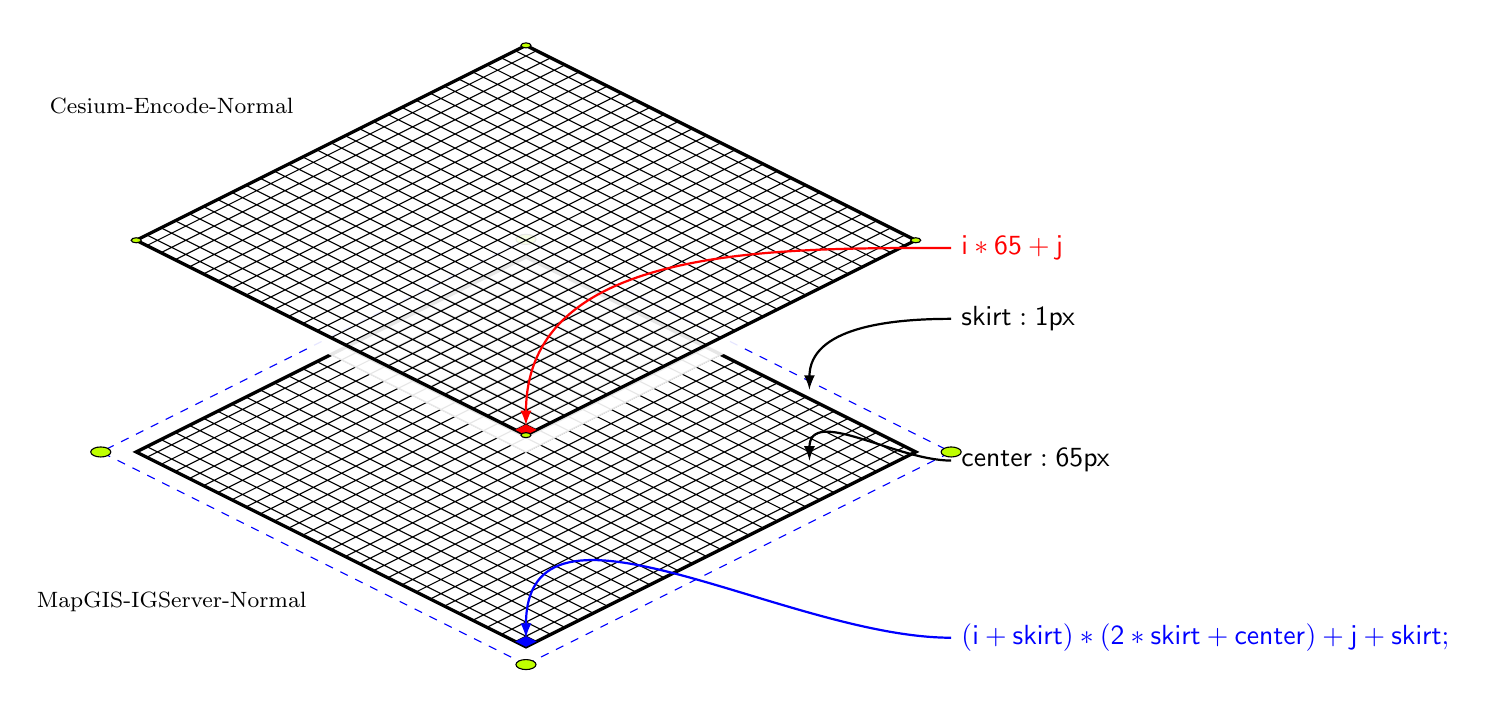
\begin{tikzpicture}[scale=.9,every node/.style={minimum size=1cm},on grid]
		
	\begin{scope}[
    	yshift=-25,every node/.append style={
    	yslant=0.5,xslant=-1},yslant=0.5,xslant=-1
    	             ]
    	\fill[white,fill opacity=.9] (0,0) rectangle (6,6);
    	\draw[step=2mm, black] (0.25,0.25) grid (5.75,5.75);
		\draw[black,very thick] (0.25,0.25) rectangle (5.75,5.75);
    	\draw[blue,dashed] (0,0) rectangle (6,6);
		\fill[blue] (0.25,0.25) rectangle (0.4,0.4);
		\draw [fill=lime](6,0) circle (.1);
		\draw [fill=lime](0,6) circle (.1);
		\draw [fill=lime](6,6) circle (.1);
		\draw [fill=lime](0,0) circle (.1);
    \end{scope}

	\begin{scope}[
    	yshift=60,every node/.append style={
    	yslant=0.5,xslant=-1},yslant=0.5,xslant=-1
    	             ]
    	\fill[white,fill opacity=.9] (0,0) rectangle (6,6);
    	\draw[step=2mm, black] (0.25,0.25) grid (5.75,5.75);
		\draw[black,very thick] (0.25,0.25) rectangle (5.75,5.75);
		\fill[red] (0.25,0.25) rectangle (0.4,0.4);
		\draw [fill=lime](5.75,0.25) circle (.05);
		\draw [fill=lime](0.25,0.25) circle (.05);
		\draw [fill=lime](0.25,5.75) circle (.05);
		\draw [fill=lime](5.75,5.75) circle (.05);
    \end{scope}	

	\draw[-latex,thick] (6,4) node[right]{$\mathsf{skirt:1px}$} to[out=180,in=90] (4,3);
	\draw[-latex,thick] (6,2) node[right]{$\mathsf{center:65px}$} to[out=180,in=90] (4,2);
	\draw[-latex,thick,red] (6,5) node[right]{$\mathsf{ i * 65 + j}$} to[out=180,in=90] (0,2.5);
	\draw[-latex,thick,blue] (6,-0.5) node[right]{$\mathsf{  (i + skirt) * (2 * skirt + center ) + j + skirt;}$} to[out=180,in=90] (0,-0.5);
	\fill[black,font=\footnotesize]
        (-5,0) node {MapGIS-IGServer-Normal}
        (-5,7) node {Cesium-Encode-Normal};
\end{tikzpicture}

\subsubsection{MapGIS地形-水面}
\begin{enumerate}
	\item MTP水面地形实际上是通过高程来计算出水面,因此数据区使用的就是地形的数据区
	\item MTP水面地形头文件结构,偏移值\textbf{offset}为\begin{equation} offset = height_{offset} = 0 (bytes)\end{equation}
	\item MTP水面地形头文件结构,存储区域为\textbf{content}为\begin{equation} content = (height \times width ) \times unit8 = (65 \times 65 ) \times 1 = 4225 (bytes) \end{equation}
\end{enumerate}

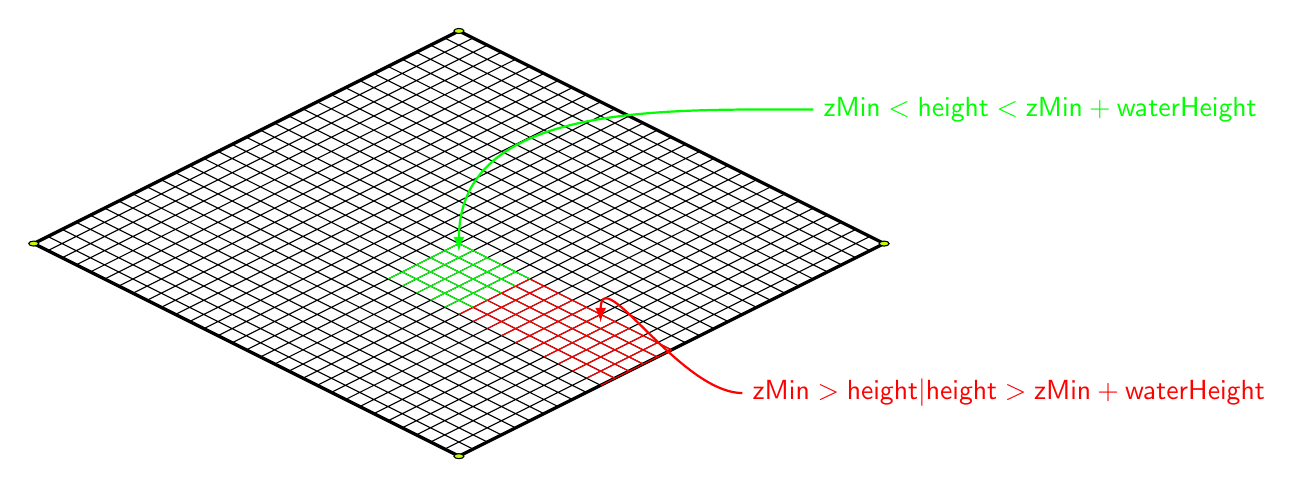
\begin{tikzpicture}[scale=.9,every node/.style={minimum size=1cm},on grid]
	\begin{scope}[
    	yshift=60,every node/.append style={
    	yslant=0.5,xslant=-1},yslant=0.5,xslant=-1
    ]
    	\fill[white,fill opacity=.9] (0,0) rectangle (6,6);
    	\draw[step=2mm, black] (0,0) grid (6,6);
		\draw[black,very thick] (0,0) rectangle (6,6);
		\draw[step=2mm, red] (2,2) grid (3,0);
		\draw[step=2mm, green] (2,2) grid (3,3);
		\draw [fill=lime](6,0) circle (.05);
		\draw [fill=lime](0,6) circle (.05);
		\draw [fill=lime](0,0) circle (.05);
		\draw [fill=lime](6,6) circle (.05);
    \end{scope}

	\draw[-latex,thick,red] (4,3) node[right]{$\mathsf{ zMin > height | height > zMin + waterHeight }$} to[out=180,in=90] (2,4);
	\draw[-latex,thick,green] (5,7) node[right]{$\mathsf{ zMin < height < zMin + waterHeight}$} to[out=180,in=90] (0,5);
\end{tikzpicture}

\begin{equation}
	f(height, zmin, waterheight) =
		\begin{cases}
			255       & \quad \text{if } zmin < height < zmin + waterheight\\
			0         & \quad \text{else } \text{其他情况}
		\end{cases}
\end{equation}

\subsubsection{Cesium地形-CTP}

\subsubsection{地形分析}
\begin{enumerate}
	\item 地形等值面(等值线)
	\item 坡度坡向分析
\end{enumerate}


\section{栅格瓦片}
\label{sec:cesium-raster}
栅格瓦片是依托于地形服务之上的一层覆盖物,如果把地形比作看不见的或者灰度高度。那么栅格就是贴合在地形上的一层覆盖物。

\begin{introduction}
	\item 等分弧秒投影瓦片
	\item Web墨卡托投影瓦片
	\item 自定义投影+自定义裁图瓦片
\end{introduction}

\subsection{核心原理}
%后面有空还是看看GlobeSurfaceTileProvider这一块的原理把%
\begin{enumerate}
	\item 首先整个地球(GlobeSurfaceTile)在初始化(initialize)的时候,会默认设置一个地形(terrainProvider)和一组栅格瓦片(imageryLayerCollection,默认至少包含一个基础的栅格瓦片底图)。
	\item 当整个环境准备好了以后,四叉树开始请求数据以后,开始准备瓦片的工作\begin{lstlisting}
		GlobeSurfaceTile.initialize = function (tile, terrainProvider, imageryLayerCollection) {
			var surfaceTile = tile.data;
			if (tile.state === QuadtreeTileLoadState.START) {
				prepareNewTile(tile, terrainProvider, imageryLayerCollection);
				tile.state = QuadtreeTileLoadState.LOADING;
			}
		};\end{lstlisting}
	\item 瓦片准备工作的步骤是先保证地形瓦片的存在,如果当前地形瓦片不存在,则向上其父级获取存在的瓦片临时作为当前地形瓦片来使用。然后遍历所有的栅格瓦片图层,每层各自请求对应的瓦片。
		\begin{lstlisting}
		function prepareNewTile(tile, terrainProvider, imageryLayerCollection) {
			var available = terrainProvider.getTileDataAvailable(tile.x, tile.y, tile.level);
		
			if (!defined(available) && defined(tile.parent)) {
				var parent = tile.parent;
				var parentSurfaceTile = parent.data;
				if (defined(parentSurfaceTile) && defined(parentSurfaceTile.terrainData)) {
					available = parentSurfaceTile.terrainData.isChildAvailable(parent.x, parent.y, tile.x, tile.y);
				}
			}
		
			if (available === false) {
				// 如果该地形瓦片是无效,立刻标记为FAILED并向上采样
				tile.data.terrainState = TerrainState.FAILED;
			}
		
			// 将栅格瓦片贴合到地形瓦片上
			for (var i = 0, len = imageryLayerCollection.length; i < len; ++i) {
				var layer = imageryLayerCollection.get(i);
				if (layer.show) {
					layer._createTileImagerySkeletons(tile, terrainProvider);
				}
			}
		}	
		\end{lstlisting}
		\item 由于地形一般都是经纬度坐标和切分方式,而栅格瓦片主流的有Web墨卡托投影(航海-电子底图)、等分弧秒投影(天地图-自然椭球)、高斯投影(自然资源-局部范围保证形变较小)甚至是自定义投影。因此不能保证每个经纬度的地形瓦片的行列号和栅格都是一一对应,因此需要有一个换算公式来进行对应的根据地形的范围来请求对应的栅格瓦片的行列号的公式。该公式就记录在createTileImagerySkeletons函数中。
		\item 上面换算公式的核心部分 一言以蔽之就是: 
		\begin{enumerate}
			\item 先通过当前栅格瓦片图层的范围和当前栅格瓦片数据源的范围进行求交分析,将空间范围缩小到有效范围内部。然后把得到的范围再和该地形瓦片的空间范围进一步求交可以得出本张瓦片(地形和栅格共同作用下)真正有效的瓦片范围。
			\item 
		\end{enumerate}
\end{enumerate}

\begin{tikzpicture}
	\begin{umlseqdiag}
		\umlobject[class=GlobeSurfaceTile]{GST}
		\umlobject[class=ImageryLayer]{IL}
		\umlobject[class=TilingScheme]{TS}
		\umlobject[class=CustomTilingScheme]{CTS}
		\begin{umlcallself}[op=initialize]{GST}
			\begin{umlcall}[op=prepareNewTile]{GST}{IL}
				\begin{umlcall}[op=createTileImagerySkeletons]{IL}{TS}	
				\end{umlcall}
			\end{umlcall}
		\end{umlcallself}
	\end{umlseqdiag}
\end{tikzpicture}


\section{M3D}
\subsection{核心入口}
	单体建筑生长.mcj
\begin{enumerate}
	\item 文件格式 \textbf{json}
	\item 文件编码 \textbf{GB2312}
\end{enumerate} 

\textbf{服务示例}
http://192.168.199.71:8089/igs/rest/services/CIMyanshi/BIM单体建筑生长V13/M3dServer

\subsubsection{索引文件MCJ}
\begin{lstlisting}
{
	"asset": "Zondy Inc.",
	"version": "2.0",
	"dataName": "高级住所模型",
	"guid": "2B444694130E4FD699A4791023735A76",
	"compressType": "0",
	"spatialReference": "WGS84",
	"treeType": "AttTree",
	"lodType": "ADD",
	"boundingVolume": {
		"boundingBox": {
			"left": 2.114275787341435,
			"top": 0.5036272461576443,
			"right": 2.1142832158691697,
			"bottom": 0.5036250037611653,
			"minHeight": -0.3499998794868589,
			"maxHeight": 13.259142253547909
		}
	},
	"position": {
		"x": 121.1392921528815,
		"y": 28.85565141287461,
		"z": 6.454571067811866
	},
	"rootNode": {
		"uri": "rootNode.json"
	},
	"fieldInfo": [ // 后期针对number型,完全可以学习cesiumlab增加一个最大最小的范围值
		{
			"alias": "alias",
			"name": "mpLayer",
			"type": "uint64",
			"size": 4
		}
	]
}
\end{lstlisting}

\subsubsection{根节点rootNode}
\begin{lstlisting}
{
    "name": "rootNode",
    "lodLevel": 0,
    "boundingVolume": { https://github.com/CesiumGS/3d-tiles/tree/main/specification#tileboundingvolume-white_check_mark
        "boundingBox": { // 既不是 Region 也不是 Box 也不是 Box 对应的转换规则可能需要说明一下,感觉像是弧度坐标
            "left": 2.114275787341435,
            "top": 0.5036272461576443,
            "right": 2.1142832158691697,
            "bottom": 0.5036250037611653,
            "minHeight": -0.3499998794868589,
            "maxHeight": 13.259142253547909
        }
    },
    "lodMode": "pixel", // 找不到3dtiles的描述,对应的枚举可能需要说明一下
    "lodType": "ADD",  // https://github.com/CesiumGS/3d-tiles/tree/main/specification#tilerefine
    "lodError": 10000.0, // https://github.com/CesiumGS/3d-tiles/tree/main/specification#tilesetgeometricerror-white_check_mark
    "childrenNode": [ // https://github.com/CesiumGS/3d-tiles/tree/main/specification#tilechildren
        {
            "boundingVolume": {
                "boundingBox": {
                    "left": 2.114275787341435,
                    "top": 0.5036272461576443,
                    "right": 2.1142832158691697,
                    "bottom": 0.5036250037611653,
                    "minHeight": -0.34999987948685887,
                    "maxHeight": 13.259142253547907
                }
            },
            "lodError": 10000.0,
            "uri": "./node/0/0.json"
        }
    ]
}
\end{lstlisting}

\subsubsection{内容节点contentNode}
\begin{figure}[!htb]
    \centering
    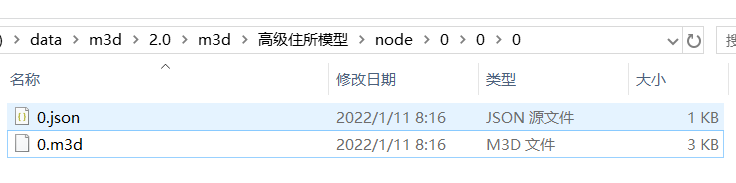
\includegraphics[width=0.9\textwidth]{./charpter2/m3d/m3d_content_json.png}
  \end{figure}
\begin{lstlisting}
	{
		"name": "2021-1-1",
		"lodLevel": 3,
		"boundingVolume": {
			"boundingBox": {
				"left": 2.114277136002482,
				"top": 0.5036251993010383,
				"right": 2.114277566540517,
				"bottom": 0.5036250263785022,
				"minHeight": 1.0846084877848626,
				"maxHeight": 4.6010056445375089
			}
		},
		"lodMode": "pixel",
		"lodType": "ADD",
		"lodError": 10000.0,
		"parentNode": {
			"uri": "../0.json"
		},
		"tileDataInfoIndex": 0,  // 这个值大部分情况是0,具体的意思是什么??
		"tileDataInfoList": [
			{
				"tileData": { // https://github.com/CesiumGS/3d-tiles/tree/main/specification#transforms
					"uri": "0.m3d"
				},
				"geometry": {
					"blobType": "glbx", // 感觉是用来做子分类的
					"uri": "./geometry/0.glbx",
					"geometryType": "Surface" // 这个的枚举可能也得说明一下了
				},
				"dataType": "Model" 
			}
		]
	}
\end{lstlisting}

\subsection{目录代码}
Source/MapGIS/M3dLayer/\textbf{MapGISM3DSet.js}
\begin{enumerate}
	\item 关键构造函数 
	\begin{lstlisting}
		// 用于访问 igs
		this._isIGServer = defaultValue(options.igserver, false);
		this._layerRenderIndex = defaultValue(options.layerRenderIndex, 0); // 渲染图层索引,这个可以具体一点不,有点抽象
		this._layerIndex = defaultValue(options.layerIndex, 0); // 图层索引(用来标识组图层的概念)
		this._gdbpUrl = defaultValue(options.gdbpUrl, ''); // 原始数据在gdb中的数据
		this._name = undefined; // 图层名
		this._guid = undefined; // 图层的guid
		this._extLayer = undefined; // 这里先为 挂接单体化预留 用来绑定单体化所用到的附加图层
		this._version = undefined;

		//fgy 20210917 update
		this._pickTextureCoordinate = defaultValue(options.pickTextureCoordinate, false);
		this._cacheState = CacheState.UNKNOW;
		this._useIDB = defaultValue(options.useIDB, false);
		this._key = '_' + this._layerRenderIndex + '_' + this.layerIndex;
		this._indexedRequest = defaultValue(options.indexedDBRequest, undefined);
		this._maxCacheLevel = defaultValue(options.maxCacheLevel, 3);
		this._pickedColor = Color.YELLOW.withAlpha(0.5);
		this._attributeNumber = 0.0;

		//ljy Pbr param
		this._pbrParam = defaultValue(options.pbrParam, undefined);

		//ljy Instances
		// 这个地方感觉是原来的文件服务 xxx.mcj做字符替换的,后面还需要吗? 这里需要一个实际数据才能明白这个逻辑
		var file_name = options.url.replace(/(.*\/)*([^.]+).*/gi, '$2');
		var FileExt = options.url.replace(/.+\./, '');
		this._sharedUrl = options.url.replace(file_name + '.' + FileExt, 'shared/');
	\end{lstlisting}
\end{enumerate}
\chapter{WebGL}

\section{材质Material}

标准的材质结构如下:
\begin{lstlisting}
    struct Material
    {
        vec3 ambient;    // 环境光照(Ambient Lighting)
        vec3 diffuse;    // 漫反射光照(Diffuse Lighting)
        vec3 specular;   // 镜面光照(Specular Lighting)
        float shininess; // 影响镜面高光的散射/半径
    };
\end{lstlisting}

Cesium的材质定义如下: 
\begin{lstlisting}
    // Source\Shaders\Builtin\Structs\material.glsl    
    struct czm_material
    {
        vec3 diffuse;    // 漫反射光照(Diffuse Lighting) vec3(0.0);
        float specular;  // 镜面光照(Specular Lighting) 0.0
        float shininess; // 影响镜面高光的散射/半径 1.0;
        vec3 normal;     // 法向量 materialInput.normalEC;
        vec3 emission;   // 发射光
        float alpha;     // 透明度
    };
    // Source\Shaders\Builtin\Structs\materialInput.glsl
    struct czm_materialInput  
    {
        float s;
        vec2 st;
        vec3 str;
        vec3 normalEC;
        mat3 tangentToEyeMatrix;
        vec3 positionToEyeEC;
        float height;
        float slope;
        float aspect;
        float uaspect;
    };
\end{lstlisting}    

Cesium的材质JavaScript对象定义如下: 
\begin{lstlisting}
// Source\Scene\Material.js
function initializeMaterial(options, result) {
    // 提取fabric中的type uniforms materials components信息
    var cachedMaterial = Material._materialCache.getMaterial(result.type);
    if (!defined(cachedMaterial)) {
        Material._materialCache.addMaterial(result.type, result);
    }

    createMethodDefinition(result); // 可以简单的认为就是按照不同的材质对struct czm_material的赋值操作
    createUniforms(result);
    createSubMaterials(result);
}
function createMethodDefinition(material) {
    var components = material._template.components;
    var source = material._template.source;
    if (defined(source)) {
        material.shaderSource += source + '\n'; // 直接使用glsl的语法
    } else {
        // 每种自定义的Material必须重写czm_getMaterial函数来实现各自的特定的参数传递
        // 其内部实现是通过解析fabric结构里面的components来自动生成对应的材质代码
        material.shaderSource += 'czm_material czm_getMaterial(czm_materialInput materialInput)\n{\n';
        // 获取从基类默认的材质结构体
        material.shaderSource += 'czm_material material = czm_getDefaultMaterial(materialInput);\n';
        if (defined(components)) {
            var isMultiMaterial = Object.keys(material._template.materials).length > 0;
            for (var component in components) {
                if (components.hasOwnProperty(component)) {
                    if (component === 'diffuse' || component === 'emission') {
                        // 针对散射光和发射光的特殊处理。如果可以复合使用不同的material就使用czm_gammaCorrect
                        // 来复合处理,否则进行常规参数的赋值处理
                        var isFusion = isMultiMaterial && isMaterialFused(components[component], material);
                        var componentSource = isFusion ? components[component] : 'czm_gammaCorrect(' + components[component] + ')';
                        material.shaderSource += 'material.' + component + ' = ' + componentSource + '; \n';
                    } else if (component === 'alpha') {
                        // 针对透明度的特殊处理,从代码分析和下面的常规参数感觉没有什么区别
                        material.shaderSource += 'material.alpha = ' + components.alpha + '; \n';
                    } else {
                        // 常规参数的赋值处理
                        material.shaderSource += 'material.' + component + ' = ' + components[component] + ';\n';
                    }
                }
            }
        }
        material.shaderSource += 'return material;\n}\n';
    }
}
function createUniform(material, uniformId) {
    // uniformType类型可能为 float、bool、channels、samplerCube、sampler2D、mat[2|3|4]、vec[2|3|4]
    var uniformType = getUniformType(uniformValue);
    // 本质上将对象化的JavaScript对象解析成glsl需要的格式
    // 并使用material._uniforms[newUniformId]来保存不同的材质的具体参数
    var newUniformId = uniformId + '_' + material._count++;
    if (uniformType === 'sampler2D') {}
    else if (uniformType === 'samplerCube') {}
    else if (uniformType.indexOf('mat') !== -1) {}
    else {}
}
\end{lstlisting}   

\section{Color举例}
\begin{lstlisting}
Material.ColorType = 'Color';
Material._materialCache.addMaterial(Material.ColorType, {
    fabric: {
        type: Material.ColorType,
        uniforms: {
            color: new Color(1.0, 0.0, 0.0, 0.5)
        },
        components: {
            diffuse: 'color.rgb',
            alpha: 'color.a'
        }
    },
    translucent: function (material) {
        return material.uniforms.color.alpha < 1.0;
    }
});
\end{lstlisting}  

% \begin{thebibliography}{9}

	\bibitem{lamport94}
	Leslie Lamport,
	\textit{\LaTeX: a document preparation system},
	Addison Wesley, Massachusetts,
	2nd edition,
	1994.

\end{thebibliography}

\nocite{*} 
\printbibliography[heading=bibliography,title=参考文献]
\appendix

\chapter{基本数学工具}


本附录包括了计量经济学中用到的一些基本数学,我们扼要论述了求和算子的各种性质,研究了线性和某些非线性方程的性质,并复习了比例和百分数。我们还介绍了一些在应用计量经济学中常见的特殊函数,包括二次函数和自然对数,前 4 节只要求基本的代数技巧,第 5 节则对微分学进行了简要回顾;虽然要理解本书的大部分内容,微积分并非必需,但在一些章末附录和第 3 篇某些高深专题中,我们还是用到了微积分。

\section{求和算子与描述统计量}

\textbf{求和算子} 是用以表达多个数求和运算的一个缩略符号,它在统计学和计量经济学分析中扮演着重要作用。如果 $\{x_i: i=1, 2, \ldots, n\}$ 表示 $n$ 个数的一个序列,那么我们就把这 $n$ 个数的和写为:

\begin{equation}
\sum_{i=1}^n x_i \equiv x_1 + x_2 +\cdots + x_n
\end{equation}



\end{document}
